% Options for packages loaded elsewhere
\PassOptionsToPackage{unicode}{hyperref}
\PassOptionsToPackage{hyphens}{url}
%
\documentclass[
  12pt,
]{article}
\usepackage{amsmath,amssymb}
\usepackage{lmodern}
\usepackage{iftex}
\ifPDFTeX
  \usepackage[T1]{fontenc}
  \usepackage[utf8]{inputenc}
  \usepackage{textcomp} % provide euro and other symbols
\else % if luatex or xetex
  \usepackage{unicode-math}
  \defaultfontfeatures{Scale=MatchLowercase}
  \defaultfontfeatures[\rmfamily]{Ligatures=TeX,Scale=1}
  \setmainfont[]{Times New Roman}
\fi
% Use upquote if available, for straight quotes in verbatim environments
\IfFileExists{upquote.sty}{\usepackage{upquote}}{}
\IfFileExists{microtype.sty}{% use microtype if available
  \usepackage[]{microtype}
  \UseMicrotypeSet[protrusion]{basicmath} % disable protrusion for tt fonts
}{}
\makeatletter
\@ifundefined{KOMAClassName}{% if non-KOMA class
  \IfFileExists{parskip.sty}{%
    \usepackage{parskip}
  }{% else
    \setlength{\parindent}{0pt}
    \setlength{\parskip}{6pt plus 2pt minus 1pt}}
}{% if KOMA class
  \KOMAoptions{parskip=half}}
\makeatother
\usepackage{xcolor}
\usepackage[margin=2.54cm]{geometry}
\usepackage{color}
\usepackage{fancyvrb}
\newcommand{\VerbBar}{|}
\newcommand{\VERB}{\Verb[commandchars=\\\{\}]}
\DefineVerbatimEnvironment{Highlighting}{Verbatim}{commandchars=\\\{\}}
% Add ',fontsize=\small' for more characters per line
\usepackage{framed}
\definecolor{shadecolor}{RGB}{248,248,248}
\newenvironment{Shaded}{\begin{snugshade}}{\end{snugshade}}
\newcommand{\AlertTok}[1]{\textcolor[rgb]{0.94,0.16,0.16}{#1}}
\newcommand{\AnnotationTok}[1]{\textcolor[rgb]{0.56,0.35,0.01}{\textbf{\textit{#1}}}}
\newcommand{\AttributeTok}[1]{\textcolor[rgb]{0.77,0.63,0.00}{#1}}
\newcommand{\BaseNTok}[1]{\textcolor[rgb]{0.00,0.00,0.81}{#1}}
\newcommand{\BuiltInTok}[1]{#1}
\newcommand{\CharTok}[1]{\textcolor[rgb]{0.31,0.60,0.02}{#1}}
\newcommand{\CommentTok}[1]{\textcolor[rgb]{0.56,0.35,0.01}{\textit{#1}}}
\newcommand{\CommentVarTok}[1]{\textcolor[rgb]{0.56,0.35,0.01}{\textbf{\textit{#1}}}}
\newcommand{\ConstantTok}[1]{\textcolor[rgb]{0.00,0.00,0.00}{#1}}
\newcommand{\ControlFlowTok}[1]{\textcolor[rgb]{0.13,0.29,0.53}{\textbf{#1}}}
\newcommand{\DataTypeTok}[1]{\textcolor[rgb]{0.13,0.29,0.53}{#1}}
\newcommand{\DecValTok}[1]{\textcolor[rgb]{0.00,0.00,0.81}{#1}}
\newcommand{\DocumentationTok}[1]{\textcolor[rgb]{0.56,0.35,0.01}{\textbf{\textit{#1}}}}
\newcommand{\ErrorTok}[1]{\textcolor[rgb]{0.64,0.00,0.00}{\textbf{#1}}}
\newcommand{\ExtensionTok}[1]{#1}
\newcommand{\FloatTok}[1]{\textcolor[rgb]{0.00,0.00,0.81}{#1}}
\newcommand{\FunctionTok}[1]{\textcolor[rgb]{0.00,0.00,0.00}{#1}}
\newcommand{\ImportTok}[1]{#1}
\newcommand{\InformationTok}[1]{\textcolor[rgb]{0.56,0.35,0.01}{\textbf{\textit{#1}}}}
\newcommand{\KeywordTok}[1]{\textcolor[rgb]{0.13,0.29,0.53}{\textbf{#1}}}
\newcommand{\NormalTok}[1]{#1}
\newcommand{\OperatorTok}[1]{\textcolor[rgb]{0.81,0.36,0.00}{\textbf{#1}}}
\newcommand{\OtherTok}[1]{\textcolor[rgb]{0.56,0.35,0.01}{#1}}
\newcommand{\PreprocessorTok}[1]{\textcolor[rgb]{0.56,0.35,0.01}{\textit{#1}}}
\newcommand{\RegionMarkerTok}[1]{#1}
\newcommand{\SpecialCharTok}[1]{\textcolor[rgb]{0.00,0.00,0.00}{#1}}
\newcommand{\SpecialStringTok}[1]{\textcolor[rgb]{0.31,0.60,0.02}{#1}}
\newcommand{\StringTok}[1]{\textcolor[rgb]{0.31,0.60,0.02}{#1}}
\newcommand{\VariableTok}[1]{\textcolor[rgb]{0.00,0.00,0.00}{#1}}
\newcommand{\VerbatimStringTok}[1]{\textcolor[rgb]{0.31,0.60,0.02}{#1}}
\newcommand{\WarningTok}[1]{\textcolor[rgb]{0.56,0.35,0.01}{\textbf{\textit{#1}}}}
\usepackage{graphicx}
\makeatletter
\def\maxwidth{\ifdim\Gin@nat@width>\linewidth\linewidth\else\Gin@nat@width\fi}
\def\maxheight{\ifdim\Gin@nat@height>\textheight\textheight\else\Gin@nat@height\fi}
\makeatother
% Scale images if necessary, so that they will not overflow the page
% margins by default, and it is still possible to overwrite the defaults
% using explicit options in \includegraphics[width, height, ...]{}
\setkeys{Gin}{width=\maxwidth,height=\maxheight,keepaspectratio}
% Set default figure placement to htbp
\makeatletter
\def\fps@figure{htbp}
\makeatother
\setlength{\emergencystretch}{3em} % prevent overfull lines
\providecommand{\tightlist}{%
  \setlength{\itemsep}{0pt}\setlength{\parskip}{0pt}}
\setcounter{secnumdepth}{5}
\usepackage{booktabs}
\usepackage{longtable}
\usepackage{array}
\usepackage{multirow}
\usepackage{wrapfig}
\usepackage{float}
\usepackage{colortbl}
\usepackage{pdflscape}
\usepackage{tabu}
\usepackage{threeparttable}
\usepackage{threeparttablex}
\usepackage[normalem]{ulem}
\usepackage{makecell}
\usepackage{xcolor}
\ifLuaTeX
  \usepackage{selnolig}  % disable illegal ligatures
\fi
\IfFileExists{bookmark.sty}{\usepackage{bookmark}}{\usepackage{hyperref}}
\IfFileExists{xurl.sty}{\usepackage{xurl}}{} % add URL line breaks if available
\urlstyle{same} % disable monospaced font for URLs
\hypersetup{
  pdftitle={Tracking COVID-19 Cases Across Different Settlement Types in New York State},
  pdfauthor={SMiltonDZouGKhalsa},
  hidelinks,
  pdfcreator={LaTeX via pandoc}}

\title{Tracking COVID-19 Cases Across Different Settlement Types in New
York State}
\usepackage{etoolbox}
\makeatletter
\providecommand{\subtitle}[1]{% add subtitle to \maketitle
  \apptocmd{\@title}{\par {\large #1 \par}}{}{}
}
\makeatother
\subtitle{\url{https://github.com/sgm22/MiltonZouKhalsa__ENV872_EDA_FinalProject}}
\author{SMiltonDZouGKhalsa}
\date{2022-11-22}

\begin{document}
\maketitle

{
\setcounter{tocdepth}{2}
\tableofcontents
}
\newpage
\listoffigures 
\newpage

\hypertarget{rationale-and-research-questions}{%
\subsection{Rationale and Research
Questions}\label{rationale-and-research-questions}}

\hypertarget{rationale}{%
\subsubsection{Rationale}\label{rationale}}

\begin{quote}
Coronavirus disease (COVID-19) is an infectious disease caused by the
severe acute respiratory syndrome coronavirus 2 (SARS-CoV-2)
(Coronavirus, n.d.). The virus is primarily spread from person to person
through respiratory droplets and as such, population density plays a
role in the transmission of the virus with many experts suggesting that
physical distancing is an effective way to combat its spread (CDCMMWR,
2020; What Is Coronavirus?, 2022). Since COVID-19 was declared a global
pandemic in March 2020 by the World Health Organization (WHO) in March
2020, there has been a resurgence in COVID-19 infections across the
globe as a result of new strains of the virus (CDC, 2020). Policy
decisions to protect human health leverages data that such as case
numbers, hospitalizations, and death resulting from COVID-19 to project
COVID-19 spread (Truelove et al., n.d.). Very few epidemiological
COVID-19 models incorporate population density explicitly even though
population density is thought to be an important factor(Hamidi et al.,
2020; Wong \& Li, 2020).
\end{quote}

\begin{quote}
In New York State, since the beginning of the pandemic there has been
over 6 million cases of COVID-19. In January 2022, the state recorded
the highest number of cases while in April 2020, it recorded the highest
record of death (Times, 2020). The density of people in New York State
varies drastically across the state with 43\% of the state's population
living in the five boroughs of New York City (New York State Tracking
Program \textbar{} Tracking \textbar{} NCEH \textbar{} CDC, 2019). Of
the 62 counties in the State, Kings County is the most populated with
over 2 million residents, while Hamilton County is the least populated
with about 4,485 residents (New York Population 2022 (Demographics,
Maps, Graphs), n.d.). With physical distancing playing an important role
in reducing the likelihood of infection, this paper explores how well
absolute population and population density predict COVID-19 case numbers
in the diversely sized New York State. Further, we explore whether the
relationship between absolute population and population density changes
among different settlement types.
\end{quote}

\begin{quote}
Settlement types are defined as population centers of humans who have
developed a long-term community in a specific area (Settlements Overview
\& Types \textbar{} What Are Settlements?, n.d.). In this study,
settlement types are classified as rural, micropolitan, and urban. We
define rural settlements as counties with a population size of less than
25,000 people, micropolitans as counties with a population size of
between 25,000 and 49,999 people, and an urban settlement as a county
with more than 50,000 people (adapted from USDA ERS - What Is Rural?,
n.d.). We hope that by better understanding the importance of population
size and density on COVID-19 prevalence and how that varies across
settlement type, we are able to better understand if population density
and/or absolute population can be used as a proxy when formulating
policy decisions around COVID-19.
\end{quote}

\hypertarget{research-questions}{%
\subsubsection{Research Questions}\label{research-questions}}

\begin{enumerate}
\def\labelenumi{\arabic{enumi}.}
\item
  What is the correlation between population density and absolute
  population and the number of COVID-19 cases across New York State?
\item
  What is the relationship between the predictor variable: settlement
  types and the response variable: cumulative COVID-19 cases?
\item
  What is the correlation between absolute population and population
  density and the number of COVID-19 tests does done? Does the stronger
  correlated relationship vary among settlement types?
\end{enumerate}

\newpage

\textbf{Set-up Working Directory, Import and Merge Data sets}

\begin{quote}
In order to answer our research question, we imported data that contains
information about New York (NY) state population size and density by
county in 2022 from the U.S. Census Bureau. This information was then
combined with data regarding number of positive COVID-19 cases, quantity
of COVID-19 tests conducted and other relevant information collected by
the New York Department of Health from March 1, 2020 to November 22,
2022.
\end{quote}

\begin{Shaded}
\begin{Highlighting}[]
\DocumentationTok{\#\#\#\#\#\#\#\#\#\#\#\#\#\#\#\#\# Set working directory \#\#\#\#\#\#\#\#\#\#\#\#\#\#\#\#\#\#\#\#\#\#\#\#\#\#\#\#\#\#\#\#}

\FunctionTok{getwd}\NormalTok{() }\CommentTok{\#Check working directory}
\end{Highlighting}
\end{Shaded}

\begin{verbatim}
## [1] "/Users/danleizou/MiltonZouKhalsa__ENV872_EDA_FinalProject3"
\end{verbatim}

\begin{Shaded}
\begin{Highlighting}[]
\CommentTok{\#Load packages}

\FunctionTok{library}\NormalTok{(rvest)}
\FunctionTok{library}\NormalTok{(tidyverse)}
\FunctionTok{library}\NormalTok{(ggplot2)}
\FunctionTok{library}\NormalTok{(ggpubr)}
\FunctionTok{library}\NormalTok{ (lubridate)}
\FunctionTok{library}\NormalTok{ (dplyr)}
\FunctionTok{library}\NormalTok{(sf)}
\FunctionTok{library}\NormalTok{ (leaflet)}
\FunctionTok{library}\NormalTok{(mapview)}
\FunctionTok{library}\NormalTok{(AER)}
\FunctionTok{library}\NormalTok{ (corrplot)}
\FunctionTok{library}\NormalTok{(RColorBrewer)}
\FunctionTok{library}\NormalTok{(knitr)}
\FunctionTok{library}\NormalTok{(MASS)}
\FunctionTok{library}\NormalTok{(kableExtra)}

\CommentTok{\#Set theme}

\NormalTok{my\_theme }\OtherTok{\textless{}{-}} \FunctionTok{theme\_bw}\NormalTok{(}\AttributeTok{base\_size =} \DecValTok{12}\NormalTok{) }\SpecialCharTok{+} 
  \FunctionTok{theme}\NormalTok{(}\AttributeTok{axis.text =} \FunctionTok{element\_text}\NormalTok{(}\AttributeTok{color =} \StringTok{"black"}\NormalTok{), }
      \AttributeTok{legend.position =} \StringTok{"top"}\NormalTok{, }\AttributeTok{legend.justification =} \StringTok{"center"}\NormalTok{) }\SpecialCharTok{+}
  \FunctionTok{theme}\NormalTok{(}\AttributeTok{plot.title =} \FunctionTok{element\_text}\NormalTok{(}\AttributeTok{hjust =} \FloatTok{0.5}\NormalTok{))}
\FunctionTok{theme\_set}\NormalTok{(my\_theme)}


\CommentTok{\#Import NY State county level COVID data (March 1, 2020 to November 22, 2022)}
\CommentTok{\#from NY Health.}

\NormalTok{ny\_covid\_dat }\OtherTok{\textless{}{-}} \FunctionTok{read.csv}\NormalTok{(}\StringTok{"./Data/Raw\_Data/NY\_COVID\_County\_Level.csv"}\NormalTok{)}

\NormalTok{ny\_covid\_dat }\CommentTok{\#View Data}
\end{Highlighting}
\end{Shaded}

\begin{verbatim}
##              County sum_new_positives sum_cumulative_no_of_positive
## 1            Albany             75450                      31527049
## 2          Allegany             10396                       4540770
## 3             Bronx            480247                     214795050
## 4            Broome             56238                      23809846
## 5    Capital Region            273064                     109650058
## 6       Cattaraugus             18648                       7739886
## 7            Cayuga             19636                       8258733
## 8  Central New York            219659                      88806060
## 9        Chautauqua             28390                      11963811
## 10          Chemung             25750                      10781572
## 11         Chenango             11387                       4672090
## 12          Clinton             21495                       7897140
## 13         Columbia             13108                       5333242
## 14         Cortland             12837                       5327906
## 15         Delaware              9685                       3752771
## 16         Dutchess             79872                      34848939
## 17             Erie            259074                     110683234
## 18            Essex              7336                       2731432
## 19     Finger Lakes            291710                     125914355
## 20         Franklin             11662                       4435661
## 21           Fulton             15935                       6306546
## 22          Genesee             16033                       6962833
## 23           Greene             10413                       4408700
## 24         Hamilton              1054                        432991
## 25         Herkimer             16859                       7020942
## 26        Jefferson             25649                       9657042
## 27            Kings            860573                     362966136
## 28            Lewis              7069                       3184476
## 29       Livingston             13875                       5860772
## 30      Long Island           1047899                     463920471
## 31          Madison             16241                       6602449
## 32       Mid-Hudson            732389                     333323687
## 33    Mohawk Valley            132784                      55129169
## 34           Monroe            184340                      81266752
## 35       Montgomery             14485                       5881959
## 36           Nassau            515433                     225331004
## 37         New York            553801                     212308156
## 38    New York City           2908643                    1224453265
## 39          Niagara             57583                      24783016
## 40    North Country             99779                      38597015
## 41           Oneida             66461                      28508629
## 42         Onondaga            137709                      55993243
## 43          Ontario             25002                      10107862
## 44           Orange            131134                      58559762
## 45          Orleans             10149                       4331454
## 46           Oswego             33236                      12623729
## 47           Otsego             12728                       4951672
## 48           Putnam             29694                      12765002
## 49           Queens            813384                     345088691
## 50       Rensselaer             40127                      15928044
## 51         Richmond            200638                      89295232
## 52         Rockland            112172                      53675641
## 53         Saratoga             59019                      22929569
## 54      Schenectady             41888                      17263319
## 55        Schoharie              6316                       2459421
## 56         Schuyler              4209                       1680264
## 57           Seneca              7336                       2910342
## 58    Southern Tier            170688                      68994999
## 59        STATEWIDE           6250706                    2668499796
## 60          Steuben             24398                      10006178
## 61     St. Lawrence             25514                      10258273
## 62          Suffolk            532466                     238589467
## 63         Sullivan             23209                       9439839
## 64            Tioga             13520                       5420118
## 65         Tompkins             25501                       8872160
## 66           Ulster             40739                      17116464
## 67           Warren             18009                       6588480
## 68       Washington             15050                       5671655
## 69            Wayne             21009                       8496183
## 70      Westchester            315569                     146918040
## 71 Western New York            374091                     159710717
## 72          Wyoming              9682                       4267904
## 73            Yates              4284                       1710253
##    sum_total_number_of_tests sum_cumulative_no_of_tests median_test_positive
## 1                    1402792                  718954664                2.43%
## 2                     248725                  135187844                1.67%
## 3                    8847438                 4167554932                2.62%
## 4                    1183008                  600726726                2.85%
## 5                    5255122                 2645289344                2.42%
## 6                     307715                  159238111                2.01%
## 7                     395524                  199795061                2.05%
## 8                    4404505                 2280257150                2.70%
## 9                     529410                  284656873               17.24%
## 10                    482115                  240229506                2.80%
## 11                    237180                  120749908                2.41%
## 12                    405091                  204944024               16.67%
## 13                    253036                  134198616                1.94%
## 14                    306593                  162613835                2.11%
## 15                    200498                  101931557                2.24%
## 16                   1482191                  765609824                2.30%
## 17                   4230697                 2209228099                2.52%
## 18                    165134                   82082708                1.87%
## 19                   5627645                 2925577026                3.11%
## 20                    217883                  104817335               19.51%
## 21                    230615                  114053436                1.69%
## 22                    274587                  141618902               20.54%
## 23                    181361                   91910867                2.54%
## 24                     20261                   10356622                0.00%
## 25                    325883                  165269120                1.80%
## 26                    407594                  191971766                2.41%
## 27                  18713833                 8370878686                2.45%
## 28                    104111                   52934295               17.14%
## 29                    285393                  152289219               21.57%
## 30                  16896935                 8450017694                3.21%
## 31                    372206                  191580055                1.89%
## 32                  13407104                 6513198457                3.08%
## 33                   2740911                 1402887769                2.05%
## 34                   3656142                 1917145805                3.25%
## 35                    223329                  114646701               17.02%
## 36                   8400598                 4188172601                2.99%
## 37                  14450368                 6672796856                2.09%
## 38                  60433651                27893288263                2.51%
## 39                    904150                  468974555               20.69%
## 40                   1940611                  970267992                2.58%
## 41                   1527340                  790655393                2.04%
## 42                   2797843                 1457537033                2.87%
## 43                    480819                  244314298                2.55%
## 44                   1968284                  904265527                3.72%
## 45                    158360                   79497423               19.67%
## 46                    532339                  268731166                1.81%
## 47                    312369                  158059656                2.10%
## 48                    490627                  243060578                2.59%
## 49                  14735060                 6902671989                2.49%
## 50                    875724                  447596670               21.30%
## 51                   3686952                 1779385800                3.25%
## 52                   2358136                 1029309794                3.01%
## 53                   1076644                  532008522                2.44%
## 54                    837442                  420680184               23.60%
## 55                    121375                   60203463               18.29%
## 56                     99602                   47465529                1.82%
## 57                    139448                   69545097               19.57%
## 58                   5973213                 3285431777                2.02%
## 59                 122900394                59623500954                3.05%
## 60                    476678                  233587858                2.50%
## 61                    620537                  323161242                2.05%
## 62                   8496337                 4261845093                3.43%
## 63                    377092                  162432097                3.13%
## 64                    234100                  115425950                2.59%
## 65                   3060032                 1825314743               10.08%
## 66                    867586                  439724686                2.64%
## 67                    339906                  161155740                2.31%
## 68                    288217                  138784081                2.00%
## 69                    383003                  193346376                2.53%
## 70                   5863188                 2968795951                2.92%
## 71                   6220697                 3257285482                2.22%
## 72                    158197                   82232070               18.97%
## 73                     91696                   45587836               14.29%
\end{verbatim}

\begin{Shaded}
\begin{Highlighting}[]
\CommentTok{\#Import NY population data (2022)}

\NormalTok{ny\_pop\_dat }\OtherTok{\textless{}{-}} \FunctionTok{read.csv}\NormalTok{(}\StringTok{"./Data/Raw\_Data/NY\_County\_Level\_Population\_Data.csv"}
\NormalTok{                       ,}\AttributeTok{stringsAsFactors =} \ConstantTok{TRUE}\NormalTok{)}

\NormalTok{ny\_pop\_dat}
\end{Highlighting}
\end{Shaded}

\begin{verbatim}
##           County pop2022 area_milessquared density_permilessquared
## 1          Kings 2782348           69.8126              39854.5289
## 2         Queens 2440412          108.7681              22436.8367
## 3  New York City 1715927           22.6558              75738.8946
## 4        Suffolk 1532434          911.7219               1680.8130
## 5          Bronx 1490164           42.0506              35437.3653
## 6         Nassau 1407022          284.8100               4940.2121
## 7    Westchester 1015525          430.5160               2358.8553
## 8           Erie  961276         1042.6977                921.9125
## 9         Monroe  762463          657.2105               1160.1504
## 10      Richmond  501151           58.1779               8614.1174
## 11      Onondaga  478414          778.4094                614.6046
## 12        Orange  407010          811.6988                501.4299
## 13      Rockland  343657          173.5039               1980.6877
## 14        Albany  316976          522.8113                606.2914
## 15      Dutchess  295595          795.6356                371.5206
## 16      Saratoga  238689          809.9962                294.6792
## 17        Oneida  231575         1212.4134                191.0033
## 18       Niagara  211906          522.3527                405.6761
## 19        Broome  198299          705.7655                280.9701
## 20        Ulster  181723         1124.2350                161.6415
## 21    Rensselaer  161470          652.4322                247.4893
## 22   Schenectady  158727          204.5787                775.8727
## 23    Chautauqua  126207         1060.2265                119.0378
## 24     Jefferson  116819         1268.6770                 92.0794
## 25        Oswego  116609          951.6435                122.5343
## 26       Ontario  113364          644.0640                176.0136
## 27  St. Lawrence  107817         2680.3786                 40.2245
## 28      Tompkins  106576          474.6493                224.5363
## 29        Putnam   97260          230.3116                422.2975
## 30       Steuben   92502         1390.5728                 66.5208
## 31         Wayne   90785          603.8264                150.3495
## 32       Chemung   83212          407.3527                204.2751
## 33       Clinton   79387         1037.8526                 76.4916
## 34      Sullivan   78840          968.1347                 81.4349
## 35   Cattaraugus   76386         1308.3601                 58.3830
## 36        Cayuga   75492          691.5917                109.1569
## 37       Madison   66930          654.8646                102.2043
## 38        Warren   65743          866.9581                 75.8318
## 39      Columbia   61264          634.7275                 96.5202
## 40    Livingston   61122          631.7622                 96.7484
## 41    Washington   60920          831.1669                 73.2945
## 42      Herkimer   59263         1411.5299                 41.9849
## 43       Genesee   58050          492.9359                117.7638
## 44        Otsego   57776         1001.7094                 57.6774
## 45        Fulton   52882          495.4601                106.7331
## 46    Montgomery   49394          403.1168                122.5302
## 47         Tioga   47921          518.6096                 92.4028
## 48        Greene   47673          647.1615                 73.6648
## 49      Franklin   46747         1629.0705                 28.6955
## 50      Chenango   46568          893.5573                 52.1153
## 51      Cortland   46303          498.7729                 92.8338
## 52      Allegany   45958         1029.3002                 44.6498
## 53      Delaware   43574         1442.4601                 30.2081
## 54       Wyoming   40207          592.7513                 67.8311
## 55       Orleans   39835          391.2631                101.8113
## 56         Essex   36983         1794.2666                 20.6118
## 57        Seneca   33526          323.7095                103.5682
## 58     Schoharie   29106          621.8189                 46.8078
## 59         Lewis   26482         1274.6433                 20.7760
## 60         Yates   24660          338.1428                 72.9278
## 61      Schuyler   17810          328.3332                 54.2437
## 62      Hamilton    5161         1717.3817                  3.0052
\end{verbatim}

\begin{Shaded}
\begin{Highlighting}[]
\CommentTok{\#Merge data sets}

\NormalTok{combined\_dat\_ny\_covid\_pop }\OtherTok{\textless{}{-}}\NormalTok{ ny\_pop\_dat }\SpecialCharTok{\%\textgreater{}\%} 
  \FunctionTok{left\_join}\NormalTok{(ny\_covid\_dat, }\AttributeTok{by =} \StringTok{"County"}\NormalTok{)}

\DocumentationTok{\#\# Add column for to classify counties into settlement types}

\NormalTok{combined\_dat\_ny\_covid\_pop }\OtherTok{\textless{}{-}}\NormalTok{ combined\_dat\_ny\_covid\_pop }\SpecialCharTok{\%\textgreater{}\%}
  \FunctionTok{mutate}\NormalTok{(}\AttributeTok{settlement\_type =} \FunctionTok{case\_when}\NormalTok{(pop2022}\SpecialCharTok{\textless{}=}\DecValTok{25000} \SpecialCharTok{\textasciitilde{}} \StringTok{\textquotesingle{}Rural\textquotesingle{}}\NormalTok{,}
                                     \DecValTok{25000}\SpecialCharTok{\textless{}=}\NormalTok{pop2022 }\SpecialCharTok{\&}\NormalTok{ pop2022}\SpecialCharTok{\textless{}}\DecValTok{50000} \SpecialCharTok{\textasciitilde{}} \StringTok{\textquotesingle{}Micropolitan\textquotesingle{}}\NormalTok{,}
\NormalTok{                                     pop2022}\SpecialCharTok{\textgreater{}=} \DecValTok{50000} \SpecialCharTok{\textasciitilde{}} \StringTok{\textquotesingle{}Urban\textquotesingle{}}\NormalTok{))}

\FunctionTok{summary}\NormalTok{(combined\_dat\_ny\_covid\_pop) }\CommentTok{\# Check data for new columns}
\end{Highlighting}
\end{Shaded}

\begin{verbatim}
##     County             pop2022        area_milessquared density_permilessquared
##  Length:62          Min.   :   5161   Min.   :  22.66   Min.   :    3.01       
##  Class :character   1st Qu.:  48289   1st Qu.: 441.55   1st Qu.:   73.02       
##  Mode  :character   Median :  86998   Median : 653.65   Median :  113.46       
##                     Mean   : 328482   Mean   : 760.09   Mean   : 3279.30       
##                     3rd Qu.: 236910   3rd Qu.:1022.40   3rd Qu.:  418.14       
##                     Max.   :2782348   Max.   :2680.38   Max.   :75738.89       
##  sum_new_positives sum_cumulative_no_of_positive sum_total_number_of_tests
##  Min.   :   1054   Min.   :4.330e+05             Min.   :   20261         
##  1st Qu.:  12905   1st Qu.:5.329e+06             1st Qu.:  240066         
##  Median :  23804   Median :9.156e+06             Median :  406342         
##  Mean   : 138799   Mean   :5.937e+07             Mean   : 2723930         
##  3rd Qu.:  64600   3rd Qu.:2.758e+07             3rd Qu.: 1462341         
##  Max.   :2908643   Max.   :1.224e+09             Max.   :60433651         
##  sum_cumulative_no_of_tests median_test_positive settlement_type   
##  Min.   :1.036e+07          Length:62            Length:62         
##  1st Qu.:1.241e+08          Class :character     Class :character  
##  Median :2.024e+08          Mode  :character     Mode  :character  
##  Mean   :1.304e+09                                                 
##  3rd Qu.:7.539e+08                                                 
##  Max.   :2.789e+10
\end{verbatim}

\newpage

\hypertarget{dataset-information}{%
\subsection{Dataset Information}\label{dataset-information}}

\begin{quote}
We acquired our 2020 to 2022 COVID-19 data from the New York Department
of Health and population data from the U.S. Census Bureau on November
24th, 2022. County names did not match between the census data and NY
Department of Health data. We wrangled our data by removing the word
``county'' from each county in the census data. In addition to the 62
counties, the NY Health Department broke counties down into smaller
sections resulting in more than 62 counties. Since we only want to work
with the original counties, we left-merged the NY health data onto the
county data on November 24th, 2022. We are using the merged version as
our main data source. Additionally on November 24th, 2022, we uploaded
the geospatial shape file that was incorporated in class for
ENV872.Using the shape file, we selected for counties in New York State.
Data types and variable types for the combined data were set on November
27th, 2022.
\end{quote}

Data Information:
\url{https://www.census.gov/library/stories/state-by-state/new-york-population-change-between-census-decade.html}
COVID-19 Variant Data \textbar{} Department of Health (ny.gov) -- (March
1, 2020, to November 22, 2022) cb\_2018\_us\_county\_20m.shp state FIPS
code 36

\textbf{Keywords}

ENV872, COVID-19, COVID, virus, virus spread, New York, New York State

\newpage

\hypertarget{exploratory-analysis-and-data-visualization}{%
\subsection{Exploratory Analysis and Data
Visualization}\label{exploratory-analysis-and-data-visualization}}

\begin{quote}
The merged data set was exploring for missing values and abnormal values
using the R functions, ``head'', ``summary'' and ``dim''. Further, to
better understand the distribution of the variables that we use in our
analysis, we plotted a series of histograms. The graphical exploration
of the distribution of the variables showed that the variables,
``sum\_cumulative\_no\_of\_positive'',
``sum\_cumulative\_no\_of\_tests'', ``pop2022'' and
``density\_permilessquared'' are right-skewed. That is, most of the data
points were located on the left side of the histograms plotted for each
variable. For improved visualization, we log transformed the variables
to get their distributions closer to a normal distribution. After each
log-transformation, we carried out Shapiro--Wilk tests to check the
normality of the transformed distributions. The p-value of each
log-transformed distribution was less than 0.05 indicating that the
evidence supported the fact that log-transformed distributions were
still not normally distributed. We also explored and visualized the
distribution of the absolute population and population density across
the various settlement types using box plots.
\end{quote}

\hypertarget{tabular-exploration}{%
\subsubsection{Tabular Exploration}\label{tabular-exploration}}

\hypertarget{graphical-exploration}{%
\subsubsection{Graphical Exploration}\label{graphical-exploration}}

\begin{Shaded}
\begin{Highlighting}[]
\CommentTok{\# Visualizing Distribution of Variables}

\DocumentationTok{\#\#\#\#\#\#\#\#\#\#\#\#\#\#\#\#\#\#\#\#\#\# COVID{-}19 Cases \#\#\#\#\#\#\#\#\#\#\#\#\#\#\#\#\#\#\#\#\#\#\#\#\#\#\#\#\#\#}

\FunctionTok{ggplot}\NormalTok{(}\AttributeTok{data =}\NormalTok{ combined\_dat\_ny\_covid\_pop, }\FunctionTok{aes}\NormalTok{(sum\_cumulative\_no\_of\_positive))}\SpecialCharTok{+}
  \FunctionTok{geom\_histogram}\NormalTok{() }\SpecialCharTok{+}
  \FunctionTok{xlab}\NormalTok{ (}\StringTok{"Cumulative Number of Positive COVID{-}19 Tests"}\NormalTok{) }\SpecialCharTok{+}
  \FunctionTok{ggtitle}\NormalTok{(}\StringTok{"Histogram of Cumulative Number of Positive COVID{-}19 Tests"}\NormalTok{)}
\end{Highlighting}
\end{Shaded}

\begin{figure}

{\centering 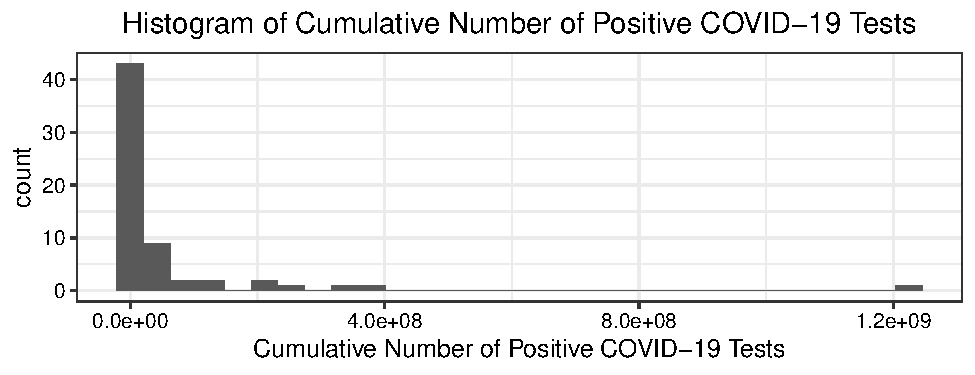
\includegraphics{EDA_Final_Group_Project_files/figure-latex/unnamed-chunk-4-1} 

}

\caption{Cumulative Number of Positive COVID-19 Tests}\label{fig:unnamed-chunk-4}
\end{figure}

\begin{Shaded}
\begin{Highlighting}[]
\DocumentationTok{\#\# Log Transform}

\FunctionTok{ggplot}\NormalTok{(}\AttributeTok{data =}\NormalTok{ combined\_dat\_ny\_covid\_pop,}
       \FunctionTok{aes}\NormalTok{(}\FunctionTok{log}\NormalTok{(sum\_cumulative\_no\_of\_positive))) }\SpecialCharTok{+}
  \FunctionTok{geom\_histogram}\NormalTok{() }\SpecialCharTok{+}
  \FunctionTok{xlab}\NormalTok{ (}\StringTok{"Log of Cumulative Number of Positive COVID{-}19 Tests"}\NormalTok{) }\SpecialCharTok{+}
  \FunctionTok{ggtitle}\NormalTok{(}\StringTok{"Histogram of Log of Cumulative Number of Positive COVID{-}19 Tests"}\NormalTok{)}
\end{Highlighting}
\end{Shaded}

\begin{figure}

{\centering 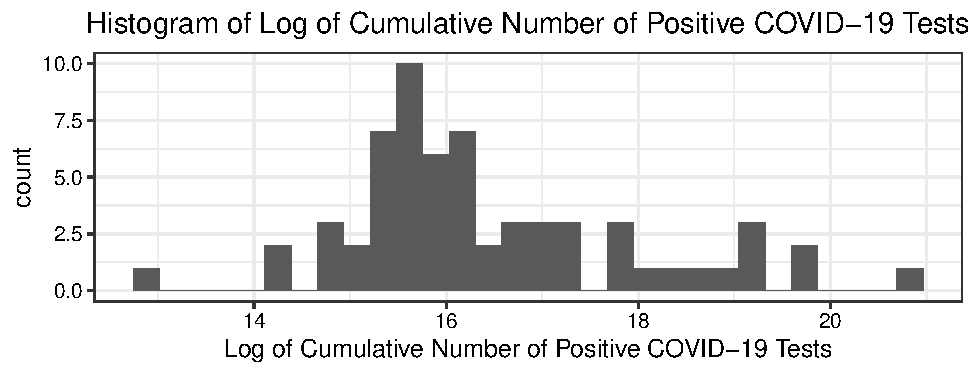
\includegraphics{EDA_Final_Group_Project_files/figure-latex/unnamed-chunk-5-1} 

}

\caption{Log of Cumulative Number of Positive COVID-19 Tests}\label{fig:unnamed-chunk-5}
\end{figure}

\begin{Shaded}
\begin{Highlighting}[]
\FunctionTok{shapiro.test}\NormalTok{(}\FunctionTok{log}\NormalTok{(combined\_dat\_ny\_covid\_pop}\SpecialCharTok{$}\NormalTok{sum\_cumulative\_no\_of\_positive)) }
\end{Highlighting}
\end{Shaded}

\begin{verbatim}
## 
##  Shapiro-Wilk normality test
## 
## data:  log(combined_dat_ny_covid_pop$sum_cumulative_no_of_positive)
## W = 0.92854, p-value = 0.001407
\end{verbatim}

\begin{Shaded}
\begin{Highlighting}[]
\CommentTok{\#Check normality}
\end{Highlighting}
\end{Shaded}

\begin{Shaded}
\begin{Highlighting}[]
\DocumentationTok{\#\#\#\#\#\#\#\#\#\#\#\#\#\#\#\#\#\#\#\#\#\#\# Number of COVID Tests Conducted \#\#\#\#\#\#\#\#\#\#\#\#\#\#\#\#\#\#\#\#\#\#\#}

\FunctionTok{ggplot}\NormalTok{(}\AttributeTok{data =}\NormalTok{ combined\_dat\_ny\_covid\_pop, }\FunctionTok{aes}\NormalTok{(sum\_cumulative\_no\_of\_tests))}\SpecialCharTok{+}
  \FunctionTok{geom\_histogram}\NormalTok{() }\SpecialCharTok{+}
  \FunctionTok{xlab}\NormalTok{ (}\StringTok{"Cumulative Number of COVID{-}19 Tests Conducted"}\NormalTok{) }\SpecialCharTok{+}
  \FunctionTok{ggtitle}\NormalTok{(}\StringTok{"Histogram of Cumulative Number of COVID{-}19 Tests Conducted"}\NormalTok{)}
\end{Highlighting}
\end{Shaded}

\begin{figure}

{\centering 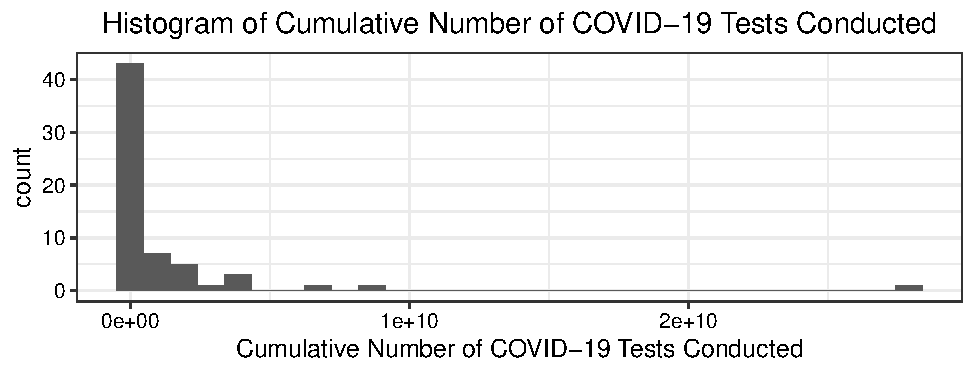
\includegraphics{EDA_Final_Group_Project_files/figure-latex/unnamed-chunk-6-1} 

}

\caption{Cumulative Number of COVID-19 Tests Conducted}\label{fig:unnamed-chunk-6}
\end{figure}

\begin{Shaded}
\begin{Highlighting}[]
\DocumentationTok{\#\# Log Transform}

\FunctionTok{ggplot}\NormalTok{(}\AttributeTok{data =}\NormalTok{ combined\_dat\_ny\_covid\_pop, }\FunctionTok{aes}\NormalTok{(}\FunctionTok{log}\NormalTok{(sum\_cumulative\_no\_of\_tests))) }\SpecialCharTok{+}
  \FunctionTok{geom\_histogram}\NormalTok{() }\SpecialCharTok{+}
  \FunctionTok{xlab}\NormalTok{ (}\StringTok{"Log of Cumulative Number of COVID{-}19 Tests Conducted"}\NormalTok{) }\SpecialCharTok{+}
  \FunctionTok{ggtitle}\NormalTok{(}\StringTok{"Histogram of Log of Cumulative Number of COVID{-}19 Tests Conducted"}\NormalTok{)}
\end{Highlighting}
\end{Shaded}

\begin{figure}

{\centering 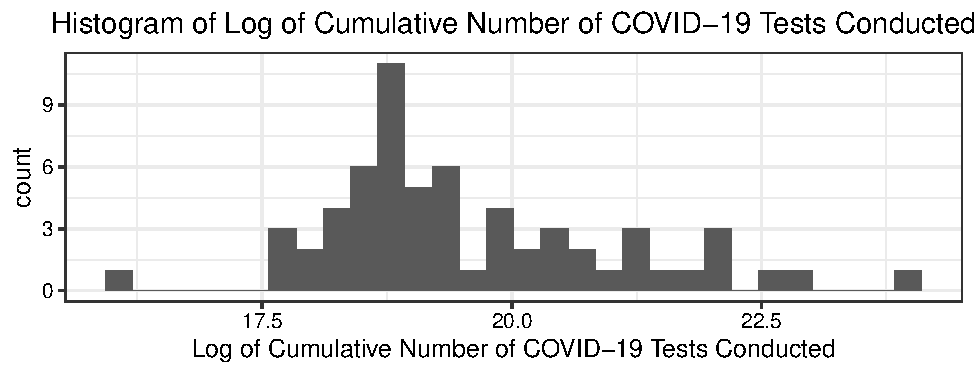
\includegraphics{EDA_Final_Group_Project_files/figure-latex/unnamed-chunk-7-1} 

}

\caption{Log of Cumulative Number of Positive COVID-19 Tests Conducted}\label{fig:unnamed-chunk-7}
\end{figure}

\begin{Shaded}
\begin{Highlighting}[]
\FunctionTok{shapiro.test}\NormalTok{(}\FunctionTok{log}\NormalTok{(combined\_dat\_ny\_covid\_pop}\SpecialCharTok{$}\NormalTok{sum\_cumulative\_no\_of\_tests))}
\end{Highlighting}
\end{Shaded}

\begin{verbatim}
## 
##  Shapiro-Wilk normality test
## 
## data:  log(combined_dat_ny_covid_pop$sum_cumulative_no_of_tests)
## W = 0.94091, p-value = 0.004985
\end{verbatim}

\begin{Shaded}
\begin{Highlighting}[]
\CommentTok{\#Check normality}
\end{Highlighting}
\end{Shaded}

\begin{Shaded}
\begin{Highlighting}[]
\DocumentationTok{\#\#\#\#\#\#\#\#\#\#\#\#\#\#\#\#\#\#\#\#\#\#\#\#\# County Population \#\#\#\#\#\#\#\#\#\#\#\#\#\#\#\#\#\#\#\#\#\#\#\#\#\#}

\FunctionTok{ggplot}\NormalTok{(}\AttributeTok{data =}\NormalTok{ combined\_dat\_ny\_covid\_pop, }\FunctionTok{aes}\NormalTok{(pop2022)) }\SpecialCharTok{+}
  \FunctionTok{geom\_histogram}\NormalTok{() }\SpecialCharTok{+}
  \FunctionTok{xlab}\NormalTok{(}\StringTok{"Absolute Population Size of Counties Across New York State 2022"}\NormalTok{) }\SpecialCharTok{+}
  \FunctionTok{ggtitle}\NormalTok{ (}\StringTok{"Histogram of Population of Counties Across New York State"}\NormalTok{)}
\end{Highlighting}
\end{Shaded}

\begin{figure}

{\centering 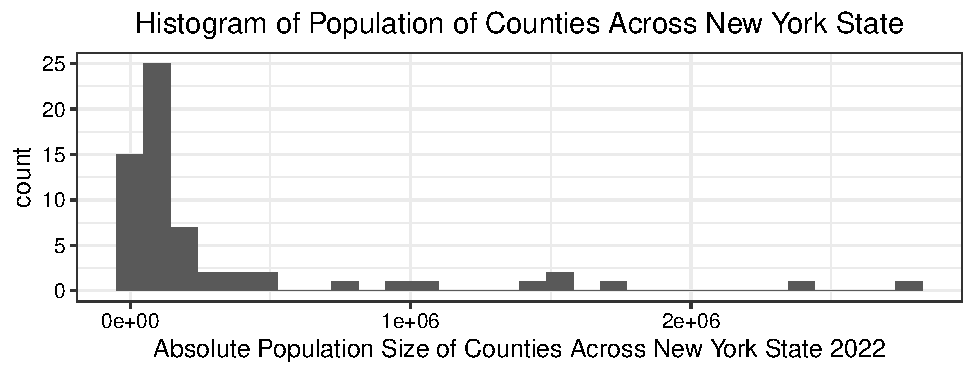
\includegraphics{EDA_Final_Group_Project_files/figure-latex/unnamed-chunk-8-1} 

}

\caption{Population of Counties Across New York State}\label{fig:unnamed-chunk-8}
\end{figure}

\begin{Shaded}
\begin{Highlighting}[]
\DocumentationTok{\#\# Log Transform}

\FunctionTok{ggplot}\NormalTok{(}\AttributeTok{data =}\NormalTok{ combined\_dat\_ny\_covid\_pop, }\FunctionTok{aes}\NormalTok{(}\FunctionTok{log}\NormalTok{(pop2022))) }\SpecialCharTok{+}
  \FunctionTok{geom\_histogram}\NormalTok{() }\SpecialCharTok{+}
  \FunctionTok{xlab}\NormalTok{(}\StringTok{"Log of Absolute Population of Counties Across New York State 2022 "}\NormalTok{) }\SpecialCharTok{+}
  \FunctionTok{ggtitle}\NormalTok{ (}\StringTok{"Log of Histogram of Population of Counties Across New York State"}\NormalTok{)}
\end{Highlighting}
\end{Shaded}

\begin{figure}

{\centering 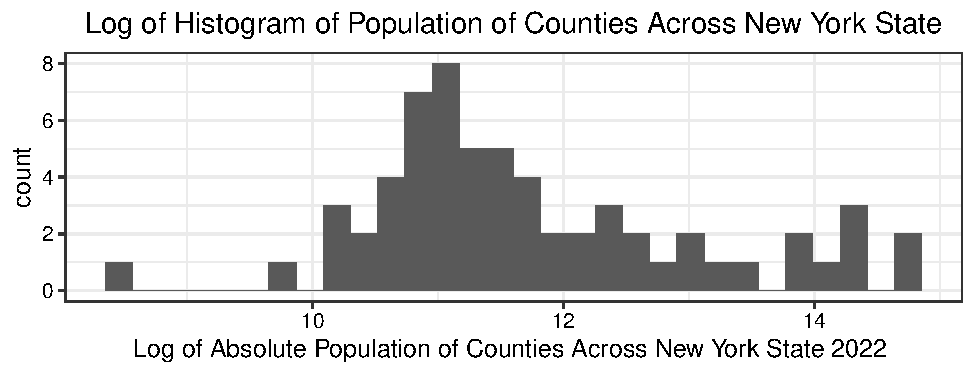
\includegraphics{EDA_Final_Group_Project_files/figure-latex/unnamed-chunk-9-1} 

}

\caption{Log of Population of Counties Across New York State}\label{fig:unnamed-chunk-9}
\end{figure}

\begin{Shaded}
\begin{Highlighting}[]
\FunctionTok{shapiro.test}\NormalTok{(}\FunctionTok{log}\NormalTok{(combined\_dat\_ny\_covid\_pop}\SpecialCharTok{$}\NormalTok{pop2022)) }\CommentTok{\#Check normaliity}
\end{Highlighting}
\end{Shaded}

\begin{verbatim}
## 
##  Shapiro-Wilk normality test
## 
## data:  log(combined_dat_ny_covid_pop$pop2022)
## W = 0.93542, p-value = 0.002814
\end{verbatim}

\begin{Shaded}
\begin{Highlighting}[]
\DocumentationTok{\#\#\#\#\#\#\#\#\#\#\#\#\#\#\#\#\#\#\#\#\#\#\#\#\#\#\#\#\#\#\#\#\#\# County Density \#\#\#\#\#\#\#\#\#\#\#\#\#\#\#\#\#\#\#\#\#\#\#\#\#\#\#\#}

\FunctionTok{ggplot}\NormalTok{(}\AttributeTok{data =}\NormalTok{ combined\_dat\_ny\_covid\_pop, }\FunctionTok{aes}\NormalTok{(density\_permilessquared)) }\SpecialCharTok{+}
  \FunctionTok{geom\_histogram}\NormalTok{() }\SpecialCharTok{+}
  \FunctionTok{xlab}\NormalTok{(}\StringTok{"Density of Counties Across New York State"}\NormalTok{) }\SpecialCharTok{+}
  \FunctionTok{ggtitle}\NormalTok{ (}\StringTok{" Histogram of Density of Counties Across New York State"}\NormalTok{)}
\end{Highlighting}
\end{Shaded}

\begin{figure}

{\centering 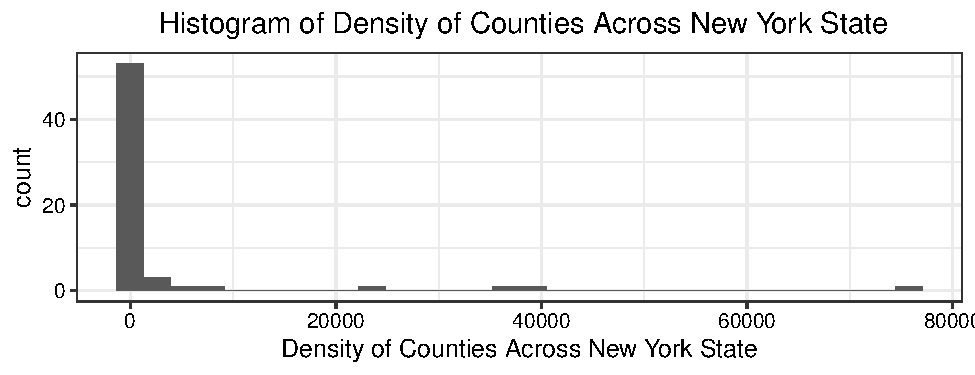
\includegraphics{EDA_Final_Group_Project_files/figure-latex/unnamed-chunk-10-1} 

}

\caption{Density of Counties Across New York State}\label{fig:unnamed-chunk-10}
\end{figure}

\begin{Shaded}
\begin{Highlighting}[]
\DocumentationTok{\#\# Log Transform}

\FunctionTok{ggplot}\NormalTok{(}\AttributeTok{data =}\NormalTok{ combined\_dat\_ny\_covid\_pop, }\FunctionTok{aes}\NormalTok{(}\FunctionTok{log}\NormalTok{(density\_permilessquared))) }\SpecialCharTok{+}
  \FunctionTok{geom\_histogram}\NormalTok{() }\SpecialCharTok{+}
  \FunctionTok{xlab}\NormalTok{(}\StringTok{"Log of Density of Counties Across New York State"}\NormalTok{) }\SpecialCharTok{+}
  \FunctionTok{ggtitle}\NormalTok{ (}\StringTok{" Log of Histogram of Density of Counties Across New York State"}\NormalTok{)}
\end{Highlighting}
\end{Shaded}

\begin{figure}

{\centering 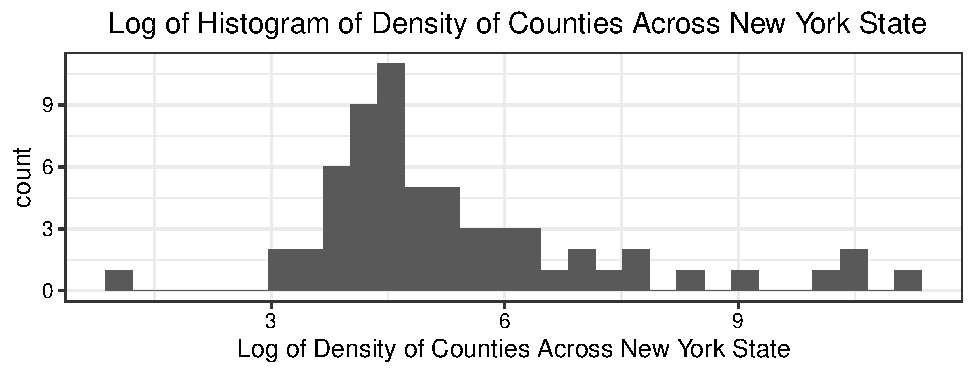
\includegraphics{EDA_Final_Group_Project_files/figure-latex/unnamed-chunk-11-1} 

}

\caption{Log of Density of Counties Across New York State}\label{fig:unnamed-chunk-11}
\end{figure}

\begin{Shaded}
\begin{Highlighting}[]
\FunctionTok{shapiro.test}\NormalTok{(}\FunctionTok{log}\NormalTok{(combined\_dat\_ny\_covid\_pop}\SpecialCharTok{$}\NormalTok{density\_permilessquared))}
\end{Highlighting}
\end{Shaded}

\begin{verbatim}
## 
##  Shapiro-Wilk normality test
## 
## data:  log(combined_dat_ny_covid_pop$density_permilessquared)
## W = 0.87808, p-value = 1.73e-05
\end{verbatim}

\begin{Shaded}
\begin{Highlighting}[]
\CommentTok{\#Check normality}
\end{Highlighting}
\end{Shaded}

\begin{Shaded}
\begin{Highlighting}[]
\DocumentationTok{\#\#\#\#\#\#\#\#\#\#\# Visualize Distribution of Predictor Variables by Settlement Type}

\FunctionTok{ggplot}\NormalTok{(}\AttributeTok{data =}\NormalTok{ combined\_dat\_ny\_covid\_pop, }\FunctionTok{aes}\NormalTok{(}\AttributeTok{x=}\NormalTok{ settlement\_type,}
                                             \AttributeTok{y=} \FunctionTok{log}\NormalTok{(density\_permilessquared),}
                                             \AttributeTok{fill =}\NormalTok{ settlement\_type))}\SpecialCharTok{+}
  \FunctionTok{geom\_boxplot}\NormalTok{() }\SpecialCharTok{+}
  \FunctionTok{ggtitle}\NormalTok{ (}\StringTok{"Log of Absolute Population Size of Counties by Settlement Type"}\NormalTok{) }\SpecialCharTok{+}
  \FunctionTok{xlab}\NormalTok{(}\StringTok{"Settlement Types"}\NormalTok{) }\SpecialCharTok{+}
  \FunctionTok{ylab}\NormalTok{(}\StringTok{"Log of Absolute Population Size 2022"}\NormalTok{)}
\end{Highlighting}
\end{Shaded}

\begin{figure}

{\centering 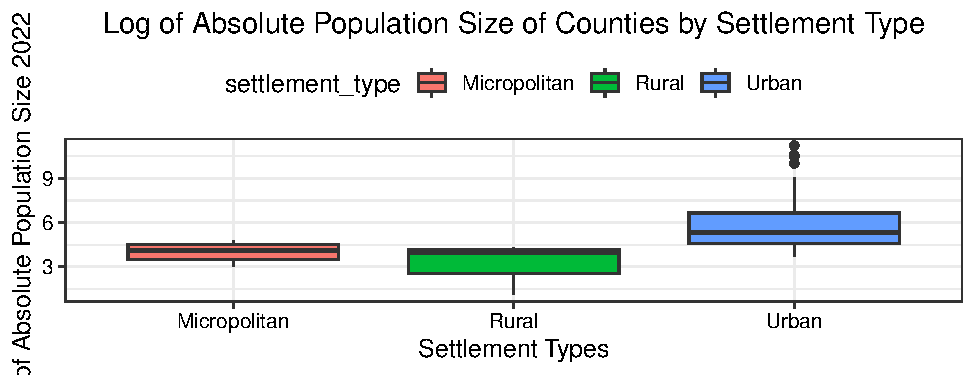
\includegraphics{EDA_Final_Group_Project_files/figure-latex/unnamed-chunk-12-1} 

}

\caption{Log of Absolute Population Size of Counties by Settlement Type}\label{fig:unnamed-chunk-12}
\end{figure}

\begin{Shaded}
\begin{Highlighting}[]
\FunctionTok{ggplot}\NormalTok{(}\AttributeTok{data =}\NormalTok{ combined\_dat\_ny\_covid\_pop,}
       \FunctionTok{aes}\NormalTok{(}\AttributeTok{x=}\NormalTok{ settlement\_type, }\AttributeTok{y=} \FunctionTok{log}\NormalTok{(pop2022), }\AttributeTok{fill =}\NormalTok{ settlement\_type))}\SpecialCharTok{+}
  \FunctionTok{geom\_boxplot}\NormalTok{() }\SpecialCharTok{+}
    \FunctionTok{ggtitle}\NormalTok{ (}\StringTok{"Log of Population Density of Counties by Settlement Type"}\NormalTok{) }\SpecialCharTok{+}
  \FunctionTok{xlab}\NormalTok{(}\StringTok{"Settlement Types"}\NormalTok{) }\SpecialCharTok{+}
  \FunctionTok{ylab}\NormalTok{(}\StringTok{"Log of Absolute Population Size 2022"}\NormalTok{)}
\end{Highlighting}
\end{Shaded}

\begin{figure}

{\centering 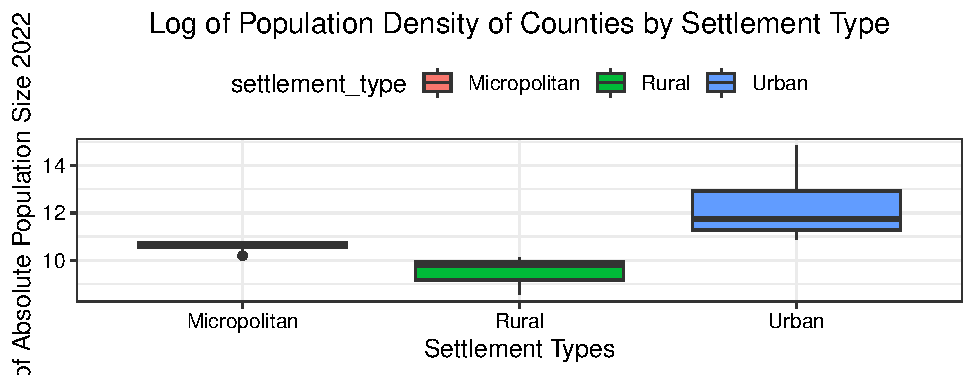
\includegraphics{EDA_Final_Group_Project_files/figure-latex/unnamed-chunk-13-1} 

}

\caption{Log of Population Density of Counties by Settlement Type}\label{fig:unnamed-chunk-13}
\end{figure}

\hypertarget{spatial-context-of-data}{%
\subsubsection{Spatial Context of Data}\label{spatial-context-of-data}}

\begin{Shaded}
\begin{Highlighting}[]
\CommentTok{\# Map of New York County Population Levels}
 
\CommentTok{\# The EPSG code of the New York counties dataset is 4269.}
\CommentTok{\#This is a geographic coordinate reference system, so it uses}
\CommentTok{\#angular coordinate units. This CRS (4269) is associated with the datum NAD83.}

\NormalTok{uscounty }\OtherTok{\textless{}{-}} \FunctionTok{st\_read}\NormalTok{(}\StringTok{\textquotesingle{}./Data/Spatial\_Files/cb\_2018\_us\_county\_20m.shp\textquotesingle{}}\NormalTok{,}
                    \AttributeTok{stringsAsFactors =} \ConstantTok{TRUE}\NormalTok{) }\SpecialCharTok{\%\textgreater{}\%}
 \FunctionTok{filter}\NormalTok{(STATEFP }\SpecialCharTok{==} \DecValTok{36}\NormalTok{)}
\end{Highlighting}
\end{Shaded}

\begin{verbatim}
## Reading layer `cb_2018_us_county_20m' from data source 
##   `/Users/danleizou/MiltonZouKhalsa__ENV872_EDA_FinalProject3/Data/Spatial_Files/cb_2018_us_county_20m.shp' 
##   using driver `ESRI Shapefile'
## Simple feature collection with 3220 features and 9 fields
## Geometry type: MULTIPOLYGON
## Dimension:     XY
## Bounding box:  xmin: -179.1743 ymin: 17.91377 xmax: 179.7739 ymax: 71.35256
## Geodetic CRS:  NAD83
\end{verbatim}

\begin{Shaded}
\begin{Highlighting}[]
\CommentTok{\# Reveal the names of the columns}
\FunctionTok{colnames}\NormalTok{(combined\_dat\_ny\_covid\_pop)}
\end{Highlighting}
\end{Shaded}

\begin{verbatim}
##  [1] "County"                        "pop2022"                      
##  [3] "area_milessquared"             "density_permilessquared"      
##  [5] "sum_new_positives"             "sum_cumulative_no_of_positive"
##  [7] "sum_total_number_of_tests"     "sum_cumulative_no_of_tests"   
##  [9] "median_test_positive"          "settlement_type"
\end{verbatim}

\begin{Shaded}
\begin{Highlighting}[]
\CommentTok{\# Join the flow data to our NWIS gage location spatial dataframe.}
\NormalTok{combined\_dat\_join }\OtherTok{\textless{}{-}} \FunctionTok{merge}\NormalTok{(}\AttributeTok{x =}\NormalTok{ uscounty,}
                          \AttributeTok{y =}\NormalTok{ combined\_dat\_ny\_covid\_pop,}
                          \AttributeTok{by.x =} \StringTok{"NAME"}\NormalTok{,}
                          \AttributeTok{by.y =} \StringTok{"County"}\NormalTok{)}
 
\CommentTok{\# Show the column names of the joined dataset.}
\FunctionTok{colnames}\NormalTok{(combined\_dat\_join)}
\end{Highlighting}
\end{Shaded}

\begin{verbatim}
##  [1] "NAME"                          "STATEFP"                      
##  [3] "COUNTYFP"                      "COUNTYNS"                     
##  [5] "AFFGEOID"                      "GEOID"                        
##  [7] "LSAD"                          "ALAND"                        
##  [9] "AWATER"                        "pop2022"                      
## [11] "area_milessquared"             "density_permilessquared"      
## [13] "sum_new_positives"             "sum_cumulative_no_of_positive"
## [15] "sum_total_number_of_tests"     "sum_cumulative_no_of_tests"   
## [17] "median_test_positive"          "settlement_type"              
## [19] "geometry"
\end{verbatim}

\begin{Shaded}
\begin{Highlighting}[]
\CommentTok{\# Show the dimensions of this joined dataset.}
\FunctionTok{dim}\NormalTok{(combined\_dat\_join)}
\end{Highlighting}
\end{Shaded}

\begin{verbatim}
## [1] 61 19
\end{verbatim}

\begin{Shaded}
\begin{Highlighting}[]
\CommentTok{\# Map the population of each New York county in 2022.}
\FunctionTok{ggplot}\NormalTok{() }\SpecialCharTok{+}
  \FunctionTok{geom\_sf}\NormalTok{(}\AttributeTok{data =}\NormalTok{ combined\_dat\_join, }\FunctionTok{aes}\NormalTok{(}\AttributeTok{fill =} \FunctionTok{log}\NormalTok{(pop2022))) }\SpecialCharTok{+}
  \FunctionTok{scale\_fill\_gradientn}\NormalTok{(}\AttributeTok{colours =} \FunctionTok{terrain.colors}\NormalTok{(}\DecValTok{10}\NormalTok{)) }\SpecialCharTok{+}
  \FunctionTok{ggtitle}\NormalTok{(}\StringTok{"COVID{-}19 in New York"}\NormalTok{,}
          \AttributeTok{subtitle =} \StringTok{"Population by County in 2022"}\NormalTok{) }\SpecialCharTok{+}
  \FunctionTok{labs}\NormalTok{(}\AttributeTok{fill =} \StringTok{\textquotesingle{}Log of Variable\textquotesingle{}}\NormalTok{)}
\end{Highlighting}
\end{Shaded}

\begin{figure}

{\centering 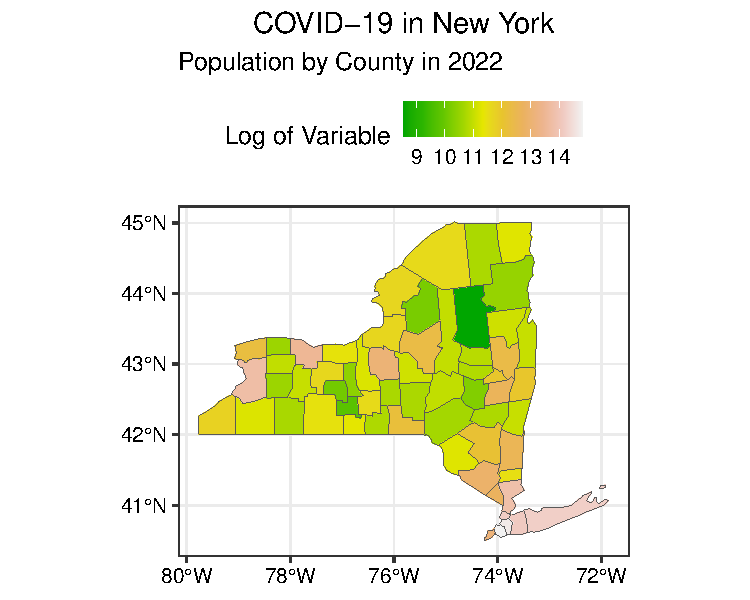
\includegraphics{EDA_Final_Group_Project_files/figure-latex/unnamed-chunk-15-1} 

}

\caption{Population of New York Counties}\label{fig:unnamed-chunk-15}
\end{figure}

\begin{Shaded}
\begin{Highlighting}[]
\CommentTok{\# Map the settlement types of each New York county in 2022.}
\FunctionTok{ggplot}\NormalTok{() }\SpecialCharTok{+}
  \FunctionTok{geom\_sf}\NormalTok{(}\AttributeTok{data =}\NormalTok{ combined\_dat\_join, }\FunctionTok{aes}\NormalTok{(}\AttributeTok{fill =}\NormalTok{ settlement\_type)) }\SpecialCharTok{+}
  \FunctionTok{ggtitle}\NormalTok{(}\StringTok{"COVID{-}19 in New York"}\NormalTok{,}
          \AttributeTok{subtitle =} \StringTok{"Settlement Types by County in 2022"}\NormalTok{) }\SpecialCharTok{+}
  \FunctionTok{labs}\NormalTok{(}\AttributeTok{fill =} \StringTok{\textquotesingle{}Settlement Types\textquotesingle{}}\NormalTok{)}
\end{Highlighting}
\end{Shaded}

\begin{figure}

{\centering 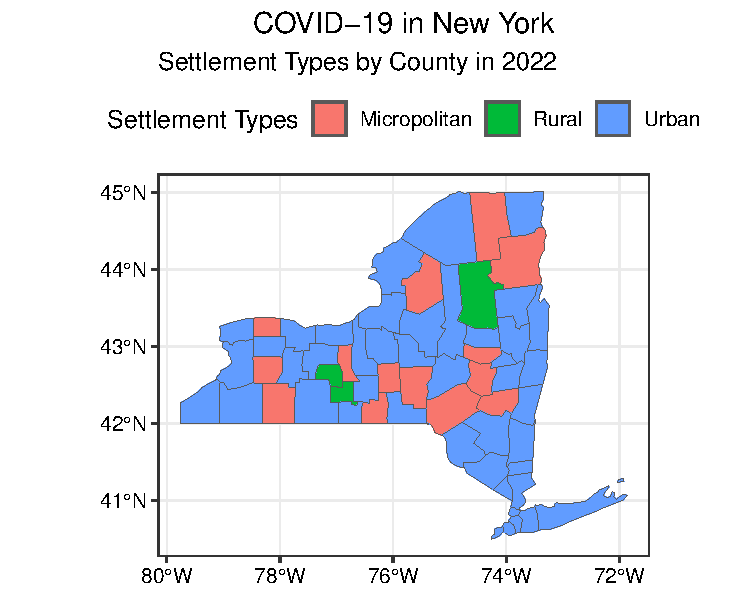
\includegraphics{EDA_Final_Group_Project_files/figure-latex/unnamed-chunk-16-1} 

}

\caption{Settlement Types of New York Counties}\label{fig:unnamed-chunk-16}
\end{figure}

\begin{Shaded}
\begin{Highlighting}[]
\CommentTok{\# Map the sum of the cumulative number of tests administered in each}
\CommentTok{\#New York county in 2022.}

\FunctionTok{ggplot}\NormalTok{() }\SpecialCharTok{+}
  \FunctionTok{geom\_sf}\NormalTok{(}\AttributeTok{data =}\NormalTok{ combined\_dat\_join,}
          \FunctionTok{aes}\NormalTok{(}\AttributeTok{fill =} \FunctionTok{log}\NormalTok{(sum\_cumulative\_no\_of\_tests))) }\SpecialCharTok{+}
  \FunctionTok{scale\_fill\_gradientn}\NormalTok{(}\AttributeTok{colours =} \FunctionTok{terrain.colors}\NormalTok{(}\DecValTok{10}\NormalTok{)) }\SpecialCharTok{+}
  \FunctionTok{ggtitle}\NormalTok{(}\StringTok{"COVID{-}19 in New York"}\NormalTok{,}
          \AttributeTok{subtitle =} \StringTok{"Cumulative Number of Tests Administered"}\NormalTok{) }\SpecialCharTok{+}
  \FunctionTok{labs}\NormalTok{(}\AttributeTok{fill =} \StringTok{\textquotesingle{}Log of Variable\textquotesingle{}}\NormalTok{)}
\end{Highlighting}
\end{Shaded}

\begin{figure}

{\centering 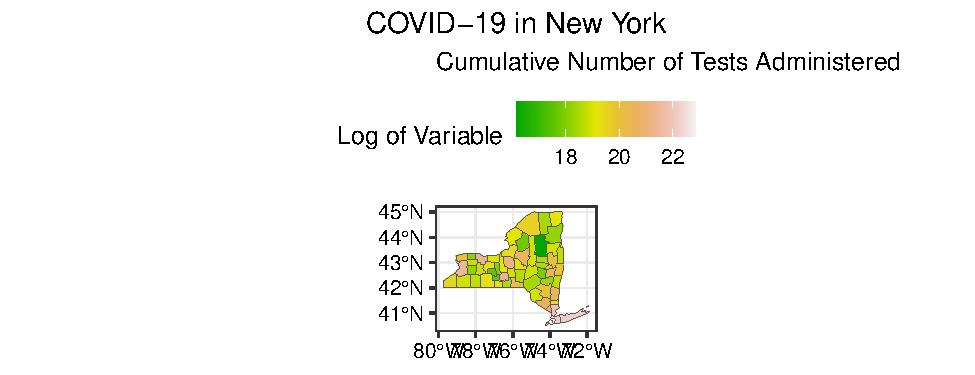
\includegraphics{EDA_Final_Group_Project_files/figure-latex/unnamed-chunk-17-1} 

}

\caption{Cumulative Number of Tests Administered in Each New York County}\label{fig:unnamed-chunk-17}
\end{figure}

\begin{Shaded}
\begin{Highlighting}[]
\CommentTok{\# Map the sum of the cumulative number of positive test results in each}
\CommentTok{\#New York county in 2022.}

\FunctionTok{ggplot}\NormalTok{() }\SpecialCharTok{+}
  \FunctionTok{geom\_sf}\NormalTok{(}\AttributeTok{data =}\NormalTok{ combined\_dat\_join,}
          \FunctionTok{aes}\NormalTok{(}\AttributeTok{fill =} \FunctionTok{log}\NormalTok{(sum\_cumulative\_no\_of\_positive))) }\SpecialCharTok{+}
  \FunctionTok{scale\_fill\_gradientn}\NormalTok{(}\AttributeTok{colours =} \FunctionTok{terrain.colors}\NormalTok{(}\DecValTok{10}\NormalTok{)) }\SpecialCharTok{+}
  \FunctionTok{ggtitle}\NormalTok{(}\StringTok{"COVID{-}19 in New York"}\NormalTok{,}
          \AttributeTok{subtitle =} \StringTok{"Cumulative Number of Positive Test Results in 2022"}\NormalTok{) }\SpecialCharTok{+}
  \FunctionTok{labs}\NormalTok{(}\AttributeTok{fill =} \StringTok{\textquotesingle{}Log of Variable\textquotesingle{}}\NormalTok{)}
\end{Highlighting}
\end{Shaded}

\begin{figure}

{\centering 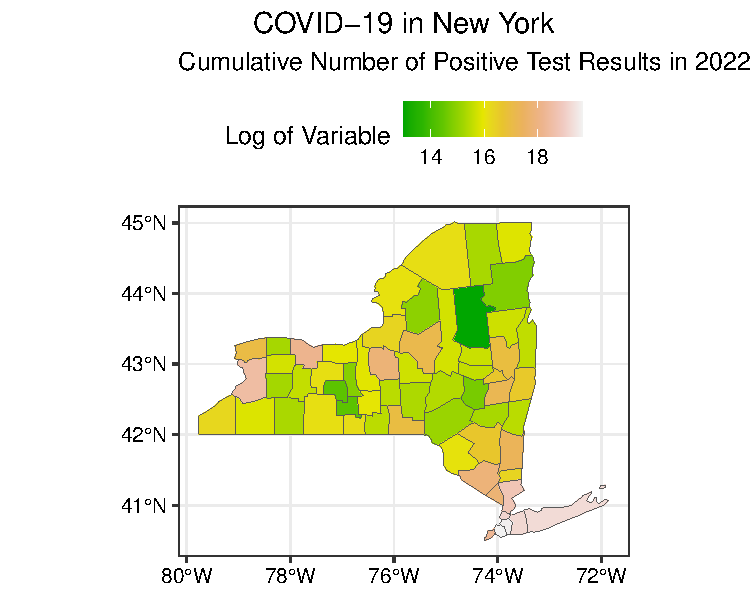
\includegraphics{EDA_Final_Group_Project_files/figure-latex/unnamed-chunk-18-1} 

}

\caption{Cumulative Number of Positive Test Results in Each New York County}\label{fig:unnamed-chunk-18}
\end{figure}

\textbf{Export Processed data}

\begin{Shaded}
\begin{Highlighting}[]
\FunctionTok{getwd}\NormalTok{() }\CommentTok{\#Check working directory}
\end{Highlighting}
\end{Shaded}

\begin{verbatim}
## [1] "/Users/danleizou/MiltonZouKhalsa__ENV872_EDA_FinalProject3"
\end{verbatim}

\begin{Shaded}
\begin{Highlighting}[]
\CommentTok{\#Full processed data set}

\FunctionTok{write.csv2}\NormalTok{(combined\_dat\_ny\_covid\_pop,}
           \StringTok{"./Data/Processed\_Data/Combined\_NY\_COVID\_Pop.csv"}\NormalTok{)}

\CommentTok{\#Collapsed data set}

\FunctionTok{write.csv2}\NormalTok{(collapsed\_dat\_settlement\_types,}
           \StringTok{"./Data/Processed\_Data/collapsed\_dat\_settlement\_types.csv"}\NormalTok{)}
\end{Highlighting}
\end{Shaded}

\newpage

\hypertarget{analysis}{%
\subsection{Analysis}\label{analysis}}

\begin{quote}
As a central question of this study is ``How well does population
density and absolute population predict COVID-19 cases?'', the predictor
variables are population density per miles squared and absolute
population while the outcome variable is sum cumulative positive number
of positive COVID-19 tests which is being used as a proxy for COVID-19
cases. Our unit of analysis is counties and settlement types depending
on the primary objective of each sub-question. Settlement types are
classified based on our definitions of rural, micropolitan, and urban
settlement types. Our hypotheses for each study question is indicated
below.
\end{quote}

\textbf{Question 1: What is the correlation between population density
and absolute population and the number of COVID-19 cases (cumulative
number of positive tests) across New York State?}

\begin{quote}
Prior to the correlation analysis, the normality of absolute population,
population density, and COVID-19 cases were examined and were determined
to not be normally distributed (see exploratory analysis). The variables
were log-transformed but were showed to still not be normally
distributed after a Shapiro-Wilk test of normality was performed. As
such, a Spearman correlation analysis for non-parametric data was
carried out. The classification of the strength of the relationship was
determined based on the value of r which ranges from 0 to 1 where r = 0
indicates no association and r = -1 or +1.
\end{quote}

\hypertarget{absolute-population-and-covid-19-cases}{%
\subsubsection{Absolute Population and COVID-19
Cases}\label{absolute-population-and-covid-19-cases}}

\emph{Hypotheses}

Null Hypothesis: As the ranks of absolute population change, the ranks
of the number of COVID-19 cases do not change.

Alternative Hypothesis: As the ranks of absolute population change, the
ranks of the number of COVID-19 cases change.

\emph{Assumptions:}

\begin{enumerate}
\def\labelenumi{\arabic{enumi}.}
\tightlist
\item
  The relationship between both variables is monotonic.
\end{enumerate}

\begin{Shaded}
\begin{Highlighting}[]
\CommentTok{\# Spearman rank correlation test as distributions are skewed}


\NormalTok{correlation\_results\_absol\_pop }\OtherTok{\textless{}{-}}
  \FunctionTok{cor.test}\NormalTok{(}\AttributeTok{x=}\FunctionTok{log}\NormalTok{(combined\_dat\_ny\_covid\_pop}\SpecialCharTok{$}\NormalTok{pop2022),}
           \AttributeTok{y=}\FunctionTok{log}\NormalTok{(combined\_dat\_ny\_covid\_pop}\SpecialCharTok{$}\NormalTok{sum\_cumulative\_no\_of\_positive),}
           \AttributeTok{method =} \StringTok{"spearman"}\NormalTok{)}
\NormalTok{correlation\_results\_absol\_pop}
\end{Highlighting}
\end{Shaded}

\begin{verbatim}
## 
##  Spearman's rank correlation rho
## 
## data:  log(combined_dat_ny_covid_pop$pop2022) and log(combined_dat_ny_covid_pop$sum_cumulative_no_of_positive)
## S = 428, p-value < 2.2e-16
## alternative hypothesis: true rho is not equal to 0
## sample estimates:
##       rho 
## 0.9892221
\end{verbatim}

\begin{Shaded}
\begin{Highlighting}[]
\CommentTok{\# Visualize plot (Log{-}transformed for better visualization)}

\FunctionTok{ggplot}\NormalTok{(combined\_dat\_ny\_covid\_pop, }\FunctionTok{aes}\NormalTok{(}\AttributeTok{x =} \FunctionTok{log}\NormalTok{(pop2022),}
                                      \AttributeTok{y =} \FunctionTok{log}\NormalTok{(sum\_cumulative\_no\_of\_positive)))}\SpecialCharTok{+}
  \FunctionTok{geom\_point}\NormalTok{() }\SpecialCharTok{+}
  \FunctionTok{ylab}\NormalTok{ (}\StringTok{"Log of COVID{-}19 Cases"}\NormalTok{) }\SpecialCharTok{+}
  \FunctionTok{xlab}\NormalTok{ (}\StringTok{"Log of Absolute Population Across Counties"}\NormalTok{) }\SpecialCharTok{+}
  \FunctionTok{ggtitle}\NormalTok{ (}\StringTok{"The Correlation Between Absolute Population }
\StringTok{           Across Counties and COVID{-}19 Cases"}\NormalTok{) }\SpecialCharTok{+}
  \FunctionTok{stat\_smooth}\NormalTok{ (}\AttributeTok{method =} \StringTok{\textquotesingle{}lm\textquotesingle{}}\NormalTok{) }\SpecialCharTok{+}
  \FunctionTok{annotate}\NormalTok{(}\StringTok{"text"}\NormalTok{,}\AttributeTok{x=}\DecValTok{9}\NormalTok{,}\AttributeTok{y=}\DecValTok{20}\NormalTok{, }\AttributeTok{label=}\NormalTok{(}\FunctionTok{paste0}\NormalTok{(}\StringTok{"R=0.99"}\NormalTok{)))}
\end{Highlighting}
\end{Shaded}

\begin{figure}
\centering
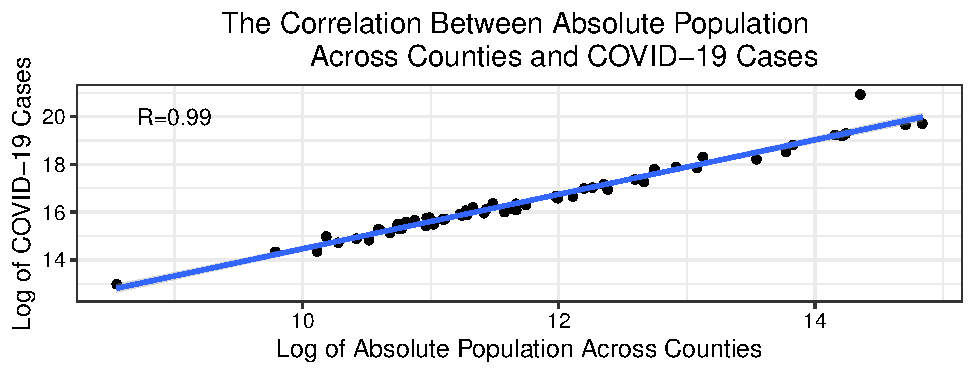
\includegraphics{EDA_Final_Group_Project_files/figure-latex/unnamed-chunk-21-1.pdf}
\caption{Correlation Between Absolute Population Across Counties and
COVID-19 Cases}
\end{figure}

\hypertarget{population-density-and-covid-19-cases}{%
\subsubsection{Population Density and COVID-19
Cases}\label{population-density-and-covid-19-cases}}

\emph{Hypotheses:}

Null Hypothesis: As the ranks of population density change, the ranks of
the number of COVID-19 cases do not change.

Alternative Hypothesis: As the ranks of population density change, the
ranks of the number of COVID-19 cases change.

\emph{Assumptions:}

\begin{enumerate}
\def\labelenumi{\arabic{enumi}.}
\tightlist
\item
  The relationship between both variables is monotonic.
\end{enumerate}

\begin{Shaded}
\begin{Highlighting}[]
\CommentTok{\# Spearman rank correlation test as distributions are skewed}


\NormalTok{correlation\_results\_pop\_density }\OtherTok{\textless{}{-}} \FunctionTok{cor.test}\NormalTok{(}\AttributeTok{x=}\FunctionTok{log}\NormalTok{(combined\_dat\_ny\_covid\_pop}\SpecialCharTok{$}\NormalTok{density\_permilessquared),}
         \AttributeTok{y=}\FunctionTok{log}\NormalTok{(combined\_dat\_ny\_covid\_pop}\SpecialCharTok{$}\NormalTok{sum\_cumulative\_no\_of\_positive),}
                                          \AttributeTok{method =} \StringTok{"spearman"}\NormalTok{)}
\NormalTok{correlation\_results\_pop\_density}
\end{Highlighting}
\end{Shaded}

\begin{verbatim}
## 
##  Spearman's rank correlation rho
## 
## data:  log(combined_dat_ny_covid_pop$density_permilessquared) and log(combined_dat_ny_covid_pop$sum_cumulative_no_of_positive)
## S = 4522, p-value < 2.2e-16
## alternative hypothesis: true rho is not equal to 0
## sample estimates:
##       rho 
## 0.8861273
\end{verbatim}

\begin{Shaded}
\begin{Highlighting}[]
\CommentTok{\# Visualize plot (Log{-}transformed for better visualization)}

\FunctionTok{ggplot}\NormalTok{(combined\_dat\_ny\_covid\_pop, }\FunctionTok{aes}\NormalTok{(}\AttributeTok{x =} \FunctionTok{log}\NormalTok{(density\_permilessquared),}
                                      \AttributeTok{y =} \FunctionTok{log}\NormalTok{(sum\_cumulative\_no\_of\_positive)))}\SpecialCharTok{+}
  \FunctionTok{geom\_point}\NormalTok{() }\SpecialCharTok{+}
  \FunctionTok{xlab}\NormalTok{ (}\StringTok{" Log of Population Density (per miles squared)"}\NormalTok{) }\SpecialCharTok{+}
  \FunctionTok{ylab}\NormalTok{ (}\StringTok{"Log of COVID{-}19 Cases"}\NormalTok{) }\SpecialCharTok{+}
  \FunctionTok{ggtitle}\NormalTok{ (}\StringTok{"The Correlation Between Population Densities}
\StringTok{           Across Counties and COVID{-}19 Cases"}\NormalTok{) }\SpecialCharTok{+}
  \FunctionTok{geom\_smooth}\NormalTok{ (}\AttributeTok{method =} \StringTok{\textquotesingle{}lm\textquotesingle{}}\NormalTok{)}\SpecialCharTok{+}
  \FunctionTok{annotate}\NormalTok{(}\StringTok{"text"}\NormalTok{,}\AttributeTok{x=}\DecValTok{3}\NormalTok{,}\AttributeTok{y=}\DecValTok{20}\NormalTok{, }\AttributeTok{label=}\NormalTok{(}\FunctionTok{paste0}\NormalTok{(}\StringTok{"R=0.89"}\NormalTok{)))}
\end{Highlighting}
\end{Shaded}

\begin{figure}

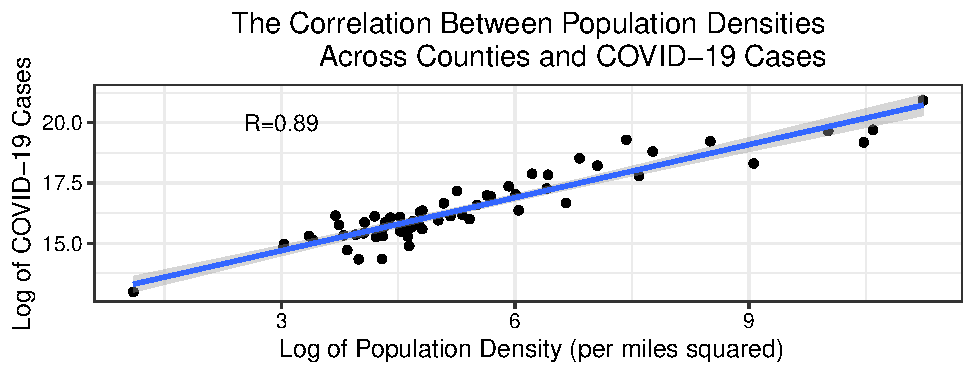
\includegraphics{EDA_Final_Group_Project_files/figure-latex/unnamed-chunk-23-1} \hfill{}

\caption{Correlation Between Population Densities Across Counties and COVID-19 Cases}\label{fig:unnamed-chunk-23}
\end{figure}

\textbf{Question 2: What is the relationship between the predictor
variable: settlement types and the response variable: cumulative
COVID-19 cases?}

\hypertarget{negative-binomial-regression}{%
\paragraph{Negative Binomial
Regression}\label{negative-binomial-regression}}

\begin{quote}
In addition to the correlation analysis, we carried out a negative
binomial regression to further understand the relationship between
settlements types (determined by levels of absolute population) and
cumulative COVID-19 cases. We used a negative binomial regression as
based on the exploratory plots, we believed that the outcome variable
can be classified as over-dispersed count data. We check our assumption
that the outcome variable,``sum\_cumulative\_no\_of\_positive'', was
overdispersed by carrying out a Poisson regression and found that the
negative binomial regression was a better fit for the data. Further, we
carried out a Chi-Square Goodness of Fit test for our negative binomial
regression model with residual deviance of 75.355 on 59 degrees of
freedom and the p-value obtained was 0.07. This means that the evidence
is more supportive of the fact that the model is a good fit.
\end{quote}

\emph{Hypotheses:}

Null Hypothesis: There is no trend between the predictor variable
(settlement types) and outcome variable (cumulative COVID-19 cases).

Alternative Hypothesis: There is a trend between the response
(settlement types) and outcome variables (cumulative COVID-19 cases).

\emph{Assumptions:}

\begin{enumerate}
\def\labelenumi{\arabic{enumi}.}
\tightlist
\item
  The response variable (COVID cases) is a count variable.
\item
  Each observation of data is independent of each other.
\item
  The mean and variance are not equal.
\end{enumerate}

\begin{Shaded}
\begin{Highlighting}[]
\DocumentationTok{\#\# Negative Binomial Regression}

\FunctionTok{summary}\NormalTok{ (modelnb }\OtherTok{\textless{}{-}}
           \FunctionTok{glm.nb}\NormalTok{(sum\_cumulative\_no\_of\_positive }\SpecialCharTok{\textasciitilde{}} \FunctionTok{factor}\NormalTok{(settlement\_type),}
                  \AttributeTok{data =}\NormalTok{ combined\_dat\_ny\_covid\_pop))}
\end{Highlighting}
\end{Shaded}

\begin{verbatim}
## 
## Call:
## glm.nb(formula = sum_cumulative_no_of_positive ~ factor(settlement_type), 
##     data = combined_dat_ny_covid_pop, init.theta = 0.6722916249, 
##     link = log)
## 
## Deviance Residuals: 
##     Min       1Q   Median       3Q      Max  
## -1.5768  -1.2869  -0.6950   0.0667   3.9330  
## 
## Coefficients:
##                              Estimate Std. Error z value Pr(>|z|)    
## (Intercept)                   15.2425     0.3260  46.763  < 2e-16 ***
## factor(settlement_type)Rural  -1.1844     0.7759  -1.526    0.127    
## factor(settlement_type)Urban   2.9602     0.3732   7.931 2.17e-15 ***
## ---
## Signif. codes:  0 '***' 0.001 '**' 0.01 '*' 0.05 '.' 0.1 ' ' 1
## 
## (Dispersion parameter for Negative Binomial(0.6723) family taken to be 1)
## 
##     Null deviance: 122.511  on 61  degrees of freedom
## Residual deviance:  75.366  on 59  degrees of freedom
## AIC: 2273.8
## 
## Number of Fisher Scoring iterations: 3
## 
## 
##               Theta:  0.672 
##           Std. Err.:  0.102 
## 
##  2 x log-likelihood:  -2265.783
\end{verbatim}

\begin{Shaded}
\begin{Highlighting}[]
\FunctionTok{par}\NormalTok{ (}\AttributeTok{mfrow =} \FunctionTok{c}\NormalTok{(}\DecValTok{2}\NormalTok{,}\DecValTok{2}\NormalTok{))}
\FunctionTok{plot}\NormalTok{(modelnb) }\CommentTok{\#Check fit}
\end{Highlighting}
\end{Shaded}

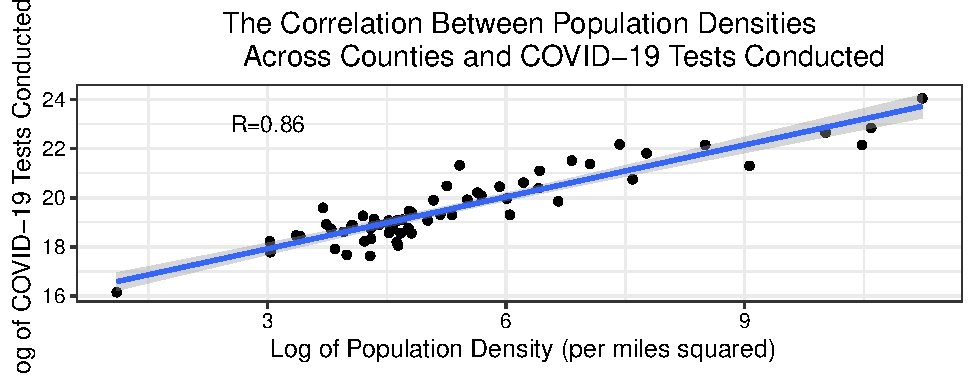
\includegraphics{EDA_Final_Group_Project_files/figure-latex/unnamed-chunk-24-1.pdf}

\begin{Shaded}
\begin{Highlighting}[]
\CommentTok{\# Test of Fitness}

\FunctionTok{pchisq}\NormalTok{(}\AttributeTok{q=}\NormalTok{modelnb}\SpecialCharTok{$}\NormalTok{deviance, }\AttributeTok{df=}\NormalTok{modelnb}\SpecialCharTok{$}\NormalTok{df.residual, }
\AttributeTok{lower.tail=}\ConstantTok{FALSE}\NormalTok{)  }\CommentTok{\#Check model fit}
\end{Highlighting}
\end{Shaded}

\begin{verbatim}
## [1] 0.0740414
\end{verbatim}

\begin{Shaded}
\begin{Highlighting}[]
\DocumentationTok{\#\# Check our assumption that a negative binomial is a better model than the}
\CommentTok{\#poisson model}

\FunctionTok{summary}\NormalTok{ (modelpoisson }\OtherTok{\textless{}{-}}
           \FunctionTok{glm}\NormalTok{(sum\_cumulative\_no\_of\_positive }\SpecialCharTok{\textasciitilde{}} \FunctionTok{factor}\NormalTok{(settlement\_type),}
               \AttributeTok{family =} \StringTok{"poisson"}\NormalTok{, }\AttributeTok{data =}\NormalTok{ combined\_dat\_ny\_covid\_pop))}
\end{Highlighting}
\end{Shaded}

\begin{verbatim}
## 
## Call:
## glm(formula = sum_cumulative_no_of_positive ~ factor(settlement_type), 
##     family = "poisson", data = combined_dat_ny_covid_pop)
## 
## Deviance Residuals: 
##    Min      1Q  Median      3Q     Max  
## -11105  -10010   -5977     168   66186  
## 
## Coefficients:
##                                Estimate Std. Error z value Pr(>|z|)    
## (Intercept)                  15.2424841  0.0001309  116408   <2e-16 ***
## factor(settlement_type)Rural -1.1844175  0.0005279   -2244   <2e-16 ***
## factor(settlement_type)Urban  2.9601778  0.0001320   22427   <2e-16 ***
## ---
## Signif. codes:  0 '***' 0.001 '**' 0.01 '*' 0.05 '.' 0.1 ' ' 1
## 
## (Dispersion parameter for poisson family taken to be 1)
## 
##     Null deviance: 1.0813e+10  on 61  degrees of freedom
## Residual deviance: 8.9559e+09  on 59  degrees of freedom
## AIC: 8955869537
## 
## Number of Fisher Scoring iterations: 6
\end{verbatim}

\begin{Shaded}
\begin{Highlighting}[]
\DocumentationTok{\#\# Summary inference: Residual deviance is much larger than degrees of}
\CommentTok{\#freedom (DF). Negative binomial plot better.}
\end{Highlighting}
\end{Shaded}

\textbf{Question 3: What is the correlation between absolute population
and population density and the number of COVID-19 tests done?}

\begin{quote}
Similar to question 1, prior to the correlation analysis, the normality
of absolute population, population density, and COVID-19 cases were
examined and were determined to not be normally distributed (see
exploratory analysis). The variables were log-transformed but were
showed to still not be normally distributed after a Shapiro-Wilk test of
normality was performed. As such, a Spearman correlation analysis for
non-parametric data was carried out. The classification of the strength
of the relationship was determined based on the value of r which ranges
from 0 to 1 where r = 0 indicates no association and r = -1 or +1.
\end{quote}

\hypertarget{absolute-population-and-covid-19-cases-1}{%
\subsubsection{Absolute Population and COVID-19
Cases}\label{absolute-population-and-covid-19-cases-1}}

\emph{Hypotheses}

Null Hypothesis: As the ranks of absolute population change, the ranks
of the number of COVID-19 tests conducted do not change.

Alternative Hypothesis: As the ranks of absolute population change, the
ranks of the number of COVID-19 tests conducted change.

\emph{Assumptions}

\begin{enumerate}
\def\labelenumi{\arabic{enumi}.}
\tightlist
\item
  The relationship between both variables is monotonic.
\end{enumerate}

\begin{Shaded}
\begin{Highlighting}[]
\CommentTok{\# Spearman rank correlation test as distributions are skewed}


\NormalTok{correlation\_results\_absol\_pop }\OtherTok{\textless{}{-}}
  \FunctionTok{cor.test}\NormalTok{(}
    \AttributeTok{x =} \FunctionTok{log}\NormalTok{(combined\_dat\_ny\_covid\_pop}\SpecialCharTok{$}\NormalTok{pop2022),}
    \AttributeTok{y =} \FunctionTok{log}\NormalTok{(combined\_dat\_ny\_covid\_pop}\SpecialCharTok{$}\NormalTok{sum\_cumulative\_no\_of\_tests),}
    \AttributeTok{method =} \StringTok{"spearman"}\NormalTok{)}
\NormalTok{correlation\_results\_absol\_pop}
\end{Highlighting}
\end{Shaded}

\begin{verbatim}
## 
##  Spearman's rank correlation rho
## 
## data:  log(combined_dat_ny_covid_pop$pop2022) and log(combined_dat_ny_covid_pop$sum_cumulative_no_of_tests)
## S = 996, p-value < 2.2e-16
## alternative hypothesis: true rho is not equal to 0
## sample estimates:
##       rho 
## 0.9749188
\end{verbatim}

\begin{Shaded}
\begin{Highlighting}[]
\CommentTok{\# Visualize plot (Log{-}transformed for better visualization)}

\FunctionTok{ggplot}\NormalTok{(combined\_dat\_ny\_covid\_pop,}
       \FunctionTok{aes}\NormalTok{(}\AttributeTok{x =} \FunctionTok{log}\NormalTok{(pop2022),}
           \AttributeTok{y =} \FunctionTok{log}\NormalTok{(sum\_cumulative\_no\_of\_tests)))}\SpecialCharTok{+}
  \FunctionTok{geom\_point}\NormalTok{() }\SpecialCharTok{+}
  \FunctionTok{ylab}\NormalTok{ (}\StringTok{"Log of COVID{-}19 Tests Conducted"}\NormalTok{) }\SpecialCharTok{+}
  \FunctionTok{xlab}\NormalTok{ (}\StringTok{"Log of Absolute Population Across Counties"}\NormalTok{) }\SpecialCharTok{+}
  \FunctionTok{ggtitle}\NormalTok{ (}\StringTok{"The Correlation Between Absolute Population }
\StringTok{           Across Counties and COVID{-}19 Tests Conducted"}\NormalTok{) }\SpecialCharTok{+}
  \FunctionTok{stat\_smooth}\NormalTok{ (}\AttributeTok{method =} \StringTok{\textquotesingle{}lm\textquotesingle{}}\NormalTok{) }\SpecialCharTok{+}
  \FunctionTok{annotate}\NormalTok{(}\StringTok{"text"}\NormalTok{,}\AttributeTok{x=}\DecValTok{9}\NormalTok{,}\AttributeTok{y=}\DecValTok{22}\NormalTok{, }\AttributeTok{label=}\NormalTok{(}\FunctionTok{paste0}\NormalTok{(}\StringTok{"R=0.97"}\NormalTok{)))}
\end{Highlighting}
\end{Shaded}

\begin{figure}

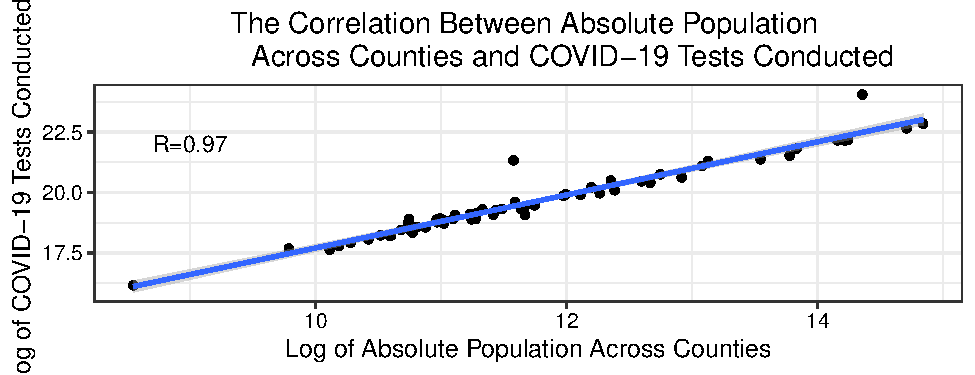
\includegraphics{EDA_Final_Group_Project_files/figure-latex/unnamed-chunk-26-1} \hfill{}

\caption{Correlation Between Absolute Population Across Counties and COVID-19 Tests Conducted}\label{fig:unnamed-chunk-26}
\end{figure}

\hypertarget{population-density-and-covid-19-cases-1}{%
\subsubsection{Population Density and COVID-19
Cases}\label{population-density-and-covid-19-cases-1}}

\emph{Hypotheses:}

Null Hypothesis: As the ranks of population density change, the ranks of
the number of COVID-19 tests conducted do not change.

Alternative Hypothesis: As the ranks of population density change, the
ranks of the number of COVID-19 tests conducted change.

\emph{Assumptions:}

\begin{enumerate}
\def\labelenumi{\arabic{enumi}.}
\tightlist
\item
  The relationship between both variables is monotonic.
\end{enumerate}

\begin{Shaded}
\begin{Highlighting}[]
\CommentTok{\# Spearman rank correlation test as distributions are skewed}


\NormalTok{correlation\_results\_pop\_density }\OtherTok{\textless{}{-}} \FunctionTok{cor.test}\NormalTok{(}
  \AttributeTok{x=} \FunctionTok{log}\NormalTok{(combined\_dat\_ny\_covid\_pop}\SpecialCharTok{$}\NormalTok{density\_permilessquared),}
  \AttributeTok{y =} \FunctionTok{log}\NormalTok{(combined\_dat\_ny\_covid\_pop}\SpecialCharTok{$}\NormalTok{sum\_cumulative\_no\_of\_tests),}
  \AttributeTok{method =} \StringTok{"spearman"}\NormalTok{)}
\NormalTok{correlation\_results\_pop\_density}
\end{Highlighting}
\end{Shaded}

\begin{verbatim}
## 
##  Spearman's rank correlation rho
## 
## data:  log(combined_dat_ny_covid_pop$density_permilessquared) and log(combined_dat_ny_covid_pop$sum_cumulative_no_of_tests)
## S = 5602, p-value < 2.2e-16
## alternative hypothesis: true rho is not equal to 0
## sample estimates:
##       rho 
## 0.8589308
\end{verbatim}

\begin{Shaded}
\begin{Highlighting}[]
\CommentTok{\# Visualize plot (Log{-}transformed for better visualization)}

\FunctionTok{ggplot}\NormalTok{(combined\_dat\_ny\_covid\_pop, }\FunctionTok{aes}\NormalTok{(}\AttributeTok{x =} \FunctionTok{log}\NormalTok{(density\_permilessquared), }\AttributeTok{y =} \FunctionTok{log}\NormalTok{(sum\_cumulative\_no\_of\_tests)))}\SpecialCharTok{+}
  \FunctionTok{geom\_point}\NormalTok{() }\SpecialCharTok{+}
  \FunctionTok{xlab}\NormalTok{ (}\StringTok{" Log of Population Density (per miles squared)"}\NormalTok{) }\SpecialCharTok{+}
  \FunctionTok{ylab}\NormalTok{ (}\StringTok{"Log of COVID{-}19 Tests Conducted"}\NormalTok{) }\SpecialCharTok{+}
  \FunctionTok{ggtitle}\NormalTok{ (}\StringTok{"The Correlation Between Population Densities}
\StringTok{           Across Counties and COVID{-}19 Tests Conducted"}\NormalTok{) }\SpecialCharTok{+}
  \FunctionTok{geom\_smooth}\NormalTok{ (}\AttributeTok{method =} \StringTok{\textquotesingle{}lm\textquotesingle{}}\NormalTok{)}\SpecialCharTok{+}
  \FunctionTok{annotate}\NormalTok{(}\StringTok{"text"}\NormalTok{,}\AttributeTok{x=}\DecValTok{3}\NormalTok{,}\AttributeTok{y=}\DecValTok{23}\NormalTok{, }\AttributeTok{label=}\NormalTok{(}\FunctionTok{paste0}\NormalTok{(}\StringTok{"R=0.86"}\NormalTok{)))}
\end{Highlighting}
\end{Shaded}

\begin{figure}

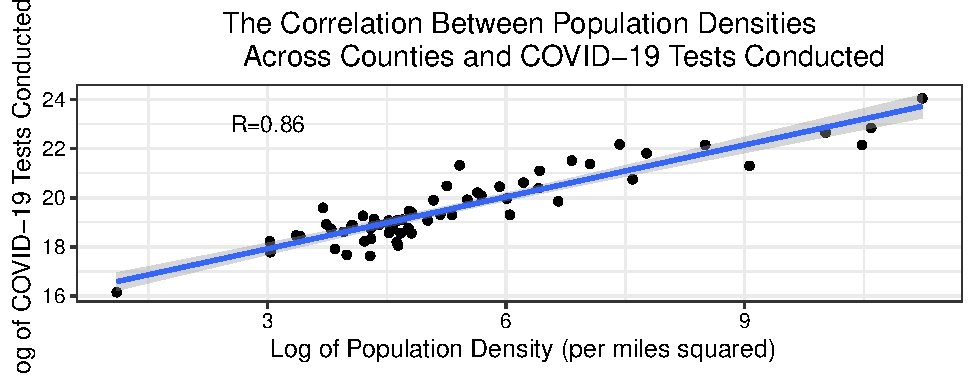
\includegraphics{EDA_Final_Group_Project_files/figure-latex/unnamed-chunk-28-1} \hfill{}

\caption{Correlation Between Absolute Population Densities Across Counties and COVID-19 Tests Conducted}\label{fig:unnamed-chunk-28}
\end{figure}

\textbf{Question 3b: Does the stronger correlated relationship vary
among settlement types?}

\hypertarget{absolute-population-and-settlement-types}{%
\paragraph{Absolute Population and Settlement
Types}\label{absolute-population-and-settlement-types}}

\begin{Shaded}
\begin{Highlighting}[]
\DocumentationTok{\#\#\# Correlation Plots by Settlement Type}

\DocumentationTok{\#\#Urban}

\NormalTok{Urban\_dat }\OtherTok{\textless{}{-}}\NormalTok{ combined\_dat\_ny\_covid\_pop }\SpecialCharTok{\%\textgreater{}\%} 
  \FunctionTok{filter}\NormalTok{(settlement\_type}\SpecialCharTok{==}\StringTok{"Urban"}\NormalTok{)}


\NormalTok{correlation\_results\_absolute\_pop\_urban }\OtherTok{\textless{}{-}}
  \FunctionTok{cor.test}\NormalTok{(}\AttributeTok{x=} \FunctionTok{log}\NormalTok{(Urban\_dat}\SpecialCharTok{$}\NormalTok{pop2022),}
           \AttributeTok{y =} \FunctionTok{log}\NormalTok{(Urban\_dat}\SpecialCharTok{$}\NormalTok{sum\_cumulative\_no\_of\_tests), }\AttributeTok{method =} \StringTok{"spearman"}\NormalTok{)}

\NormalTok{correlation\_results\_absolute\_pop\_urban}
\end{Highlighting}
\end{Shaded}

\begin{verbatim}
## 
##  Spearman's rank correlation rho
## 
## data:  log(Urban_dat$pop2022) and log(Urban_dat$sum_cumulative_no_of_tests)
## S = 632, p-value < 2.2e-16
## alternative hypothesis: true rho is not equal to 0
## sample estimates:
##       rho 
## 0.9583663
\end{verbatim}

\begin{Shaded}
\begin{Highlighting}[]
\DocumentationTok{\#\# Micropolitan}

\NormalTok{Micropolitan\_dat }\OtherTok{\textless{}{-}}\NormalTok{ combined\_dat\_ny\_covid\_pop }\SpecialCharTok{\%\textgreater{}\%} 
  \FunctionTok{filter}\NormalTok{(settlement\_type}\SpecialCharTok{==}\StringTok{"Micropolitan"}\NormalTok{)}


\NormalTok{correlation\_results\_absolute\_pop\_microp }\OtherTok{\textless{}{-}}
  \FunctionTok{cor.test}\NormalTok{(}\AttributeTok{x=} \FunctionTok{log}\NormalTok{(Micropolitan\_dat}\SpecialCharTok{$}\NormalTok{pop2022),}
           \AttributeTok{y =} \FunctionTok{log}\NormalTok{(Micropolitan\_dat}\SpecialCharTok{$}\NormalTok{sum\_cumulative\_no\_of\_tests),}
          \AttributeTok{method =} \StringTok{"spearman"}\NormalTok{)}

\NormalTok{correlation\_results\_absolute\_pop\_microp}
\end{Highlighting}
\end{Shaded}

\begin{verbatim}
## 
##  Spearman's rank correlation rho
## 
## data:  log(Micropolitan_dat$pop2022) and log(Micropolitan_dat$sum_cumulative_no_of_tests)
## S = 106, p-value = 0.002105
## alternative hypothesis: true rho is not equal to 0
## sample estimates:
##      rho 
## 0.767033
\end{verbatim}

\begin{Shaded}
\begin{Highlighting}[]
\DocumentationTok{\#\#Rural}

\NormalTok{Rural\_dat }\OtherTok{\textless{}{-}}\NormalTok{ combined\_dat\_ny\_covid\_pop }\SpecialCharTok{\%\textgreater{}\%} 
  \FunctionTok{filter}\NormalTok{(settlement\_type}\SpecialCharTok{==}\StringTok{"Rural"}\NormalTok{)}


\NormalTok{correlation\_results\_absolute\_pop\_rural }\OtherTok{\textless{}{-}} 
  \FunctionTok{cor.test}\NormalTok{(}\AttributeTok{x=} \FunctionTok{log}\NormalTok{(Rural\_dat}\SpecialCharTok{$}\NormalTok{pop2022),}
           \AttributeTok{y =} \FunctionTok{log}\NormalTok{(Rural\_dat}\SpecialCharTok{$}\NormalTok{sum\_cumulative\_no\_of\_tests), }\AttributeTok{method =} \StringTok{"spearman"}\NormalTok{)}

\NormalTok{correlation\_results\_absolute\_pop\_rural}
\end{Highlighting}
\end{Shaded}

\begin{verbatim}
## 
##  Spearman's rank correlation rho
## 
## data:  log(Rural_dat$pop2022) and log(Rural_dat$sum_cumulative_no_of_tests)
## S = 2, p-value = 1
## alternative hypothesis: true rho is not equal to 0
## sample estimates:
## rho 
## 0.5
\end{verbatim}

\hypertarget{visualization-of-3b}{%
\paragraph{Visualization of 3b}\label{visualization-of-3b}}

\begin{Shaded}
\begin{Highlighting}[]
\FunctionTok{ggplot}\NormalTok{(combined\_dat\_ny\_covid\_pop, }\FunctionTok{aes}\NormalTok{(}\AttributeTok{x =} \FunctionTok{log}\NormalTok{(pop2022),}
                                      \AttributeTok{y =} \FunctionTok{log}\NormalTok{(sum\_cumulative\_no\_of\_positive)))}\SpecialCharTok{+}
  \FunctionTok{geom\_point}\NormalTok{() }\SpecialCharTok{+} 
  \FunctionTok{ylab}\NormalTok{ (}\StringTok{"Log of Cumulative Number of COVID{-}19 Cases"}\NormalTok{) }\SpecialCharTok{+}
  \FunctionTok{xlab}\NormalTok{ (}\StringTok{"Absolute Population (2022)"}\NormalTok{)}\SpecialCharTok{+}
  \FunctionTok{facet\_wrap}\NormalTok{(}\FunctionTok{vars}\NormalTok{(settlement\_type)) }
\end{Highlighting}
\end{Shaded}

\begin{figure}

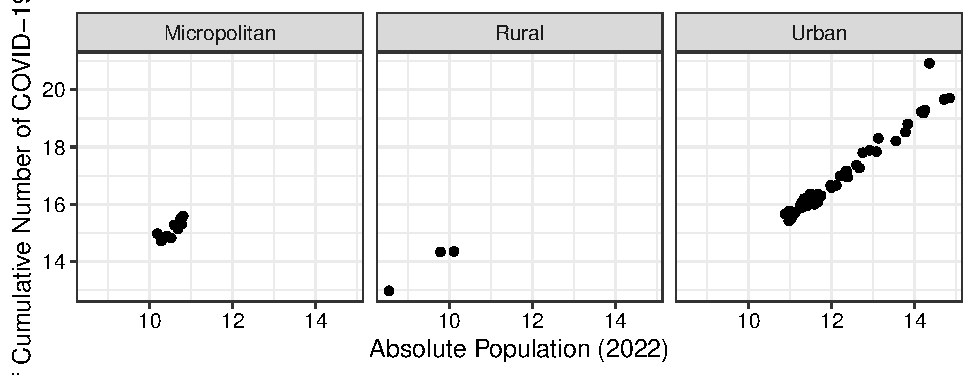
\includegraphics{EDA_Final_Group_Project_files/figure-latex/unnamed-chunk-30-1} \hfill{}

\caption{Log of Cumulative COVID-19 Cases Across Settlement Types}\label{fig:unnamed-chunk-30}
\end{figure}

\newpage

\hypertarget{summary-and-conclusions}{%
\subsection{Summary and Conclusions}\label{summary-and-conclusions}}

\hypertarget{general-overview-of-data}{%
\paragraph{General Overview of Data}\label{general-overview-of-data}}

\begin{quote}
The most populous county in New York State according to the information
we obtained from the US Census Bureau is Kings County which has a
population of over 2.7 million people. Meanwhile, the least populous
county was Hamilton county with a little over 5000 residents. Despite
Kings County have the most residents in the state, New York City was the
most densely populated county - with 75,739 residents per squared miles.
In addition to being the least populated county, Hamilton was the least
dense of the 62 counties in New York State.
\end{quote}

\hypertarget{correlation-between-absolute-population-and-population-density-with-covid-19-cases}{%
\paragraph{Correlation between Absolute Population and Population
Density with COVID-19
Cases}\label{correlation-between-absolute-population-and-population-density-with-covid-19-cases}}

\begin{quote}
We set out to answer our central question, ``How well absolute
population and population density predict COVID-19 case numbers in the
diversely sized New York State?'' by first examining the correlation
between population density and absolute population and the number of
COVID-19 cases across New York. In both cases of population density and
absolute population, after performing a Spearman correlation for both
variables we had a p-value of 2.2e-16, which suggests that the
correlated relationship was statistically significant. This means we
have sufficient evidence to reject our null hypothesis that as the ranks
of absolute populationand population density change, the ranks of the
number of COVID-19 cases do not change and instead accept our
alternative hypothesis that as the ranks of absolute population and
population density change, the ranks of the number of COVID-19 cases
does change. It is also demonstrated in the visualized plots that there
is indeed a positive correlation between the variables as the R-squared
value for the population density plot was 0.89 and 0.99 for the absolute
population plot. Both show a strong correlation, but it is stronger with
absolute population.
\end{quote}

\hypertarget{association-between-covid-19-cases-and-settlement-types}{%
\paragraph{Association between COVID-19 Cases and Settlement
Types}\label{association-between-covid-19-cases-and-settlement-types}}

\begin{quote}
In the second question, we examined the relationship between our
predictor variable (settlement types) and response variable (cumulative
COVID-19 cases). We did not control for potential confounding factors
which limits the strength of the conclusions we are able to draw from
this analysis. After performing a negative binomial regression, we
observed that the variable level, rural, has a coefficient of -1.1844
which is associated with a p-value of 0.127. This means that when
compared to the reference settlement level, micropolitan, the difference
in the logs of the expected counts is expected to be 1.1844 lower for
rural when compared to micropolitan. However, with a p-value of 0.127,
the evidence is more supportive of the fact that this relationship is
not significant. Meanwhile, we observed that when compared to the
reference level, micropolitan, the difference in the logs of expected
counts is expected to be 7.931 higher for urban settlements. The p-value
obtained for this association is less than 0.05 indicating that the
evidence is more supportive of the fact that this association is
statistically significant.
\end{quote}

\hypertarget{correlation-between-absolute-population-and-population-density-with-number-of-covid-19-tests-conducted}{%
\paragraph{Correlation between Absolute Population and Population
Density with Number of COVID-19 Tests
Conducted}\label{correlation-between-absolute-population-and-population-density-with-number-of-covid-19-tests-conducted}}

\begin{quote}
In our last question, we examined the correlation between absolute
population and population density and the number of COVID-19 tests
conducted in New York. Similar to the results of our first question,
after performing a Spearman rank correlation test with both absolute
population and population density we found that both had a p-value of
2.2e-16, indicating that the correlated relationship was statistically
significant.Therefore, we have sufficient evidence to reject both null
hypotheses that as ranks of absolute populationand population density
change, the the ranks of the number of COVID-19 tests conducted do not
change. Instead, we accept our alternative hypotheses that as ranks of
absolute population and population density change, the ranks of the
number of COVID-19 tests conducted does change. This is also shown in
our visualized plots, with the absolute population plot having an
R-squared value of 0.97 and the population density plot having an
R-squared value of 0.86. Both show a strong correlation, but it is
stronger with absolute population.
\end{quote}

\begin{quote}
After determining that the correlation between absolute population and
number of COVID-19 tests conducted is stronger, we examined within those
parameters to see if this correlation varies among settlement types. We
performed the Spearman rank correlation test on all three settlement
types. Urban settlements had a p-value of 2.2e-16 and an R-squared value
of 0.96, micropolitan settlements had a p-value of 0.002 and an
R-squared value of 0.77, and rural settlements had a p-value of 1 and an
R-squared value of 0.5. Two of the p-values show that the correlated
relationships are significant, and rural didn't have a significant
correlated relationship. The correlation is strongest with urban
settlements. However, we do acknowledge that the rural settlements only
had 3 data points, which is much fewer than the amount of data of
micropolitan and urban settlements.
\end{quote}

\hypertarget{conclusion}{%
\subsection{Conclusion}\label{conclusion}}

\begin{quote}
In conclusion, we do see a strong correlation between both absolute
population and population density and the number of COVID-19 cases in
New York, as well as the relationship between both absolute population
and population density and the number of COVID-19 tests conducted in New
York. The absolute population correlation to the number of COVID-19
tests conducted was the stronger relationship. It is important for us to
know the correlation between COVID-19 cases and settlement type so we
can be better informed about what factors influence the spread of
infectious diseases for the future.
\end{quote}

\newpage

\hypertarget{references}{%
\subsection{References}\label{references}}

\begin{enumerate}
\def\labelenumi{\arabic{enumi}.}
\item
  CDC. (2020, February 11). COVID-19 and Your Health. Centers for
  Disease Control and Prevention.
  \url{https://www.cdc.gov/coronavirus/2019-ncov/your-health/reinfection.html}
\item
  CDCMMWR. (2020). Geographic Differences in COVID-19 Cases, Deaths, and
  Incidence---United States, February 12--April 7, 2020. MMWR. Morbidity
  and Mortality Weekly Report, 69.
  \url{https://doi.org/10.15585/mmwr.mm6915e4}
\item
  Coronavirus. (n.d.). Retrieved March 14, 2022, from
  \url{https://www.who.int/westernpacific/health-topics/coronavirus}
\item
  Hamidi, S., Sabouri, S., \& Ewing, R. (2020). Does Density Aggravate
  the COVID-19 Pandemic? Journal of the American Planning Association,
  86(4), 495--509. \url{https://doi.org/10.1080/01944363.2020.1777891}
\item
  New York Population 2022 (Demographics, Maps, Graphs). (n.d.).
  Retrieved December 10, 2022, from
  \url{https://worldpopulationreview.com/states/new-york-population}
\item
  New York State Tracking Program \textbar{} Tracking \textbar{} NCEH
  \textbar{} CDC. (2019, February 20).
  \url{https://www.cdc.gov/nceh/tracking/profiles/New_York_State_Profile.htm}
\item
  Settlements Overview \& Types \textbar{} What are Settlements? - Video
  \& Lesson Transcript. (n.d.). Study.Com. Retrieved December 10, 2022,
  from
  \url{https://study.com/learn/lesson/settlements-overview-types.html}
\item
  Times, T. N. Y. (2020, April 1). New York Coronavirus Map and Case
  Count. The New York Times.
  \url{https://www.nytimes.com/interactive/2021/us/new-york-covid-cases.html}
\item
  Truelove, S., Smith, C. P., Qin, M., Mullany, L. C., Borchering, R.
  K., Lessler, J., Shea, K., Howerton, E., Contamin, L., Levander, J.,
  Kerr, J., Hochheiser, H., Kinsey, M., Tallaksen, K., Wilson, S., Shin,
  L., Rainwater-Lovett, K., Lemairtre, J.
\item
  C., Dent, J., \ldots{} Viboud, C. (n.d.). Projected resurgence of
  COVID-19 in the United States in July---December 2021 resulting from
  the increased transmissibility of the Delta variant and faltering
  vaccination. ELife, 11, e73584.
  \url{https://doi.org/10.7554/eLife.73584}
\item
  USDA ERS - What is Rural? (n.d.). Retrieved November 27, 2022, from
  \url{https://www.ers.usda.gov/topics/rural-economy-population/rural-classifications/what-is-rural.aspx}
\item
  What Is Coronavirus? (2022, July 29).
  \url{https://www.hopkinsmedicine.org/health/conditions-and-diseases/coronavirus}
\item
  Wong, D. W. S., \& Li, Y. (2020). Spreading of COVID-19: Density
  matters. PLOS ONE, 15(12), e0242398.
  \url{https://doi.org/10.1371/journal.pone.0242398}
\end{enumerate}

\end{document}
